\section{Les 3: equivalentierelaties, monoïden en groepen}

Dit hoofdstuk bevat alles wat besproken is in les 3, alsook de ontbrekende delen van hoofdstuk 2 uit de cursustekst.

\subsection{Equivalentierelaties en partities}

\SimpleHeading{Het kernidee}

Er bestaat een \textbf{1-op-1 verband} tussen equivalentierelaties op een verzameling en partities van die verzameling. Dit is misschien wel het belangrijkste idee van dit hoofdstuk.

\textbf{Intuïtief:} een equivalentierelatie zegt "deze elementen tellen voor mij als hetzelfde". Een partitie deelt de verzameling op in vakjes. Deze twee dingen zijn fundamenteel dezelfde structuur, vanuit twee perspectieven bekeken.

\textbf{\underline{Voorbeelden:}}
\begin{itemize}
    \item \inlinetext{$=$} is een equivalentierelatie, want:
    \begin{equation*}
        \begin{cases}
            a=a \\
            a=b \Rightarrow b=a \\
            a=b \text{ en } b=c \Rightarrow a=c
        \end{cases}
    \end{equation*}
    \item $A = \{\text{mensen}\}$ "hebben dezelfde moeder"
    \item Zij $m \in \mathbb{Z}_{\ge 1}$ en $A=\mathbb{Z}$, dan is de volgende relatie een equivalentierelatie:
    \begin{equation*}
        R = \{(a,b) \in \mathbb{Z}^2 \mid a \equiv b \;\text{ mod }\;m\}
    \end{equation*}
    Ter verduidelijking van de notatie:
    \begin{equation*}
        \begin{gathered}
            a \equiv b \;\text{ mod }\;m \\
            \Updownarrow \\
            m\text{ is een deler van } a - b\\
            \text{of}\\
            m \mid a - b \\
            \Updownarrow \\
            a \text{ en } b \text{ hebben dezelfde rest bij deling door }m
        \end{gathered}
    \end{equation*}
\end{itemize}

\begin{barbox}[ProcessBlue][gray!1]
    \textcolor{ProcessBlue}{\textbf{Notatie:}} Voor een equivalentierelatie schrijven we meestal \inlinetext{$\sim$} ipv. $R$.

    $\to$ dus $a \sim a$, enz.
\end{barbox}

\begin{nicedefinition}*[Equivalentieklasse]\label{def:l3_equivalentieklasse}
    Zij $A$ een verzameling en $\sim$ een equivalentierelatie op $A$.\newline
    Zij $a \in A$, dan geldt:
    \nextpart[]*
    \begin{equation}
        \bar{a} = \{x \in A \mid x \sim a\} \qedtag
    \end{equation}
    $\bar{a}$ wordt de \textcolor{PineGreen!75!black}{\textbf{equivalentieklasse}} van $a$ genoemd.
\end{nicedefinition}
Elke $b \in \bar{a}$ wordt een \inlinetext{representant}[Goldenrod!66] (= "vertegenwoordiger" in de cursustekst) van $\bar{a}$ genoemd.

Door reflexiviteit is het element $a$ zelf ook een vertegenwoordiger van $\bar{a}$ want:
\begin{equation*}
    a \in A \qquad \text{en} \quad \underbrace{a \sim a}_{reflexiviteit} \Rightarrow \quad a \in \bar{a}
\end{equation*}

\textbf{\underbar{Merk op:}} als $b \in \bar{a}$ geldt steeds:
\begin{equation}\label{eq:l3_bar_b_is_bar_a}
    \bar{b} = \bar{a}
\end{equation}
want omdat $b \in \bar{a}$, geldt per definitie van de equivalentieklasse (\Cref{def:l3_equivalentieklasse}) dat
\begin{equation*}
    b \sim a
\end{equation*}
We tonen nu aan dat $\bar{a} = \bar{b}$. Neem eerst $x \in \bar{b}$. Dan geldt:
\begin{equation*}
    x \sim b
\end{equation*}
Aangezien $b \sim a$, volgt uit transitiviteit:
\begin{equation*}
    \begin{gathered}
        x \sim b \quad \text{en} \quad b \sim a \\
        \Downarrow \\
        x \sim a
    \end{gathered}
\end{equation*}
Dus $x \in \bar{a}$. Hieruit volgt dan dat: $\quad \bar{b} \subseteq \bar{a}\qquad$ (1).

Omgekeerd, neem $x \in \bar{a}$. Dan geldt:
\begin{equation*}
    x \sim a
\end{equation*}
Omdat $b \sim a$, geldt door symmetrie ook:
\begin{equation*}
    a \sim b
\end{equation*}
Uit transitiviteit volgt dan:
\begin{equation*}
    \begin{gathered}
        x \sim a \quad \text{en} \quad a \sim b \\
        \Downarrow \\
        x \sim b
    \end{gathered}
\end{equation*}
Dus $x \in \bar{b}$. Hieruit volgt dat: $\quad \bar{a} \subseteq \bar{b} \qquad$ (2).

Uit (1) en (2) volgt dan $\bar{b} = \bar{a}$.

\begin{niceexample}*
    \nextpart[]*
    Voor $\ldots \equiv \dots \text{ mod } m$, zijn de equivalentieklassen van de vorm:
    \begin{equation*}
        \bar{a} = \{\;a + km \mid k \in \mathbb{Z}\;\}
    \end{equation*}
    Dit zijn alle gehele getallen die dezelfde rest hebben bij deling door $m$.

    \vspace{0.25cm}

    Elke element van deze vorm ($a+km$) is een \textcolor{orange!75!black}{\textbf{representant}}.

    \vspace{0.25cm}

    \textcolor{orange!75!black}{\textbf{\underbar{Meer nog:}}} elke equivalentieklasse heeft een unieke representant in $\{0,1,\dots,m-1\}$. Inderdaad: bij deling door $m$ heeft elk geheel getal een unieke rest $r$ met $0 \le r < m$, en deze rest $r$ is de unieke representant van de equivalentieklasse binnen deze verzameling.

    \vspace{0.25cm}

    Bijvoorbeeld voor modulo 5:
    \begin{equation*}
        \bar{2} = \{\dots, -8, -3, 2, 7, 12, \dots\}
    \end{equation*}
\end{niceexample}

\begin{niceproperty}*
    \nextpart[Representanten]*
    kunnen nooit tot dezelfde equivalentieklasse behoren.
\end{niceproperty}

\SimpleHeading{Partitie}

\begin{nicelemma}
    Zij $A$ een verzameling en "$\sim$" een equivalentierelatie op $A$. Dan vormen de equivalentieklassen een \textcolor{purple!50!black}{\textbf{partitie}} van $A$.
\end{nicelemma}

\begin{center}
\resizebox{0.5\textwidth}{!}{%
    \begin{tikzpicture}[
    stripe/.style={MidnightBlue, line width=1.2pt},
    circleA/.style={MidnightBlue, line width=1.4pt},
    note/.style={black, font=\large},
    arrow/.style={black, line width=1.2pt, -{Stealth[length=2.5mm]}}
]

% Circle A
\draw[circleA] (0,0) circle (2);

% Label A
\node[note] at (1.15,2.35) {$A$};

% Clip stripes to inside the circle
\begin{scope}
    \clip (0,0) circle (2);

    % Alle lijnen zijn perfect parallel: richting 45 graden, dus vector (4,4)
    \foreach \c in {-3.25,-1.95,-0.65,0.65,1.95,3.25} {
        \draw[stripe] (-3,\c-3) -- (3,\c+3);
    }

\end{scope}

% Gestippelde indicatie, ook onder hoek van 45 graden
\draw[MidnightBlue, dotted, line width=1.5pt]
    (0.55,-0.45) -- (0.85,-0.75);

% Arrow and text on the right
\draw[arrow] (2.6,1.2) -- (3.5,1.2);
\node[note, right] at (3.55,1.2) {disjunct};

\end{tikzpicture}
}
\end{center}

\begin{nicedefinition}*[Partitie]
    \nextpart[Definitie:]*
    $P \subset 2^A$ ($2^A$ is de verzameling van alle deelverzamelingen van $A$) is een partitie van $A$ \emph{asa}
    \begin{enumerate}
        \item $\emptyset \notin P$ -- geen enkele klasse is leeg
        \item $\forall \; c_1, c_2 \in P \;:\; c_1 \cap c_2 = \emptyset$ of $c_1 = c_2$ -- verschillende klassen overlappen niet
        \item $\bigcup_{c \in P}c = A$ -- de unie van alle klassen is $A$
    \end{enumerate}
\end{nicedefinition}

\textbf{\underbar{Bewijs:}}
\begin{enumerate}
    \item $\forall \; a \in A \;:\; \underbrace{a \sim a}_{\text{reflexiviteit}} \Rightarrow a \in \bar{a}$ Dus geen lege equivalentieklassen.
    \item \begin{equation*}
        \begin{gathered}
            \text{Stel } x \in \bar{a} \cap \bar{b} \\
            \Downarrow \\
            x \in \bar{a} \quad \text{en} \quad x \in \bar{b} \\
            \Downarrow \\
            \bar{x} = \bar{a} \quad \text{en} \quad \bar{x} = \bar{b} \\
            \Downarrow \\
            \bar{x} = \bar{a} = \bar{b}
        \end{gathered}
    \end{equation*}

    \item idem aan 1.
\end{enumerate}

\SimpleHeading{Van partitie naar equivalentierelatie en omgekeerd}

\begin{nicetheorem}* \label{theorem:ER_naar_E_klassen}
    \nextpart[]*
    Elke equivalentierelatie "$\sim$" ($R$ in cursus) op $A$ geeft een partitie $P=\{\bar{a}\}$ ($P=\{R_x\}$ in cursus) waarbij $\bar{a} = \{y \in A \mid y \sim a\}$ de \textcolor{red!66!black}{\textbf{equivalentieklasse}} van $a$ is. Let op: $\{\bar{a}\}$ is de verzameling van alle equivalentieklassen, en dus een verzameling van deelverzamelingen, wat de partitie is, niet $\bar{a}$!
    
    \vspace{0.5cm}

    Omgekeerd: Zij $P$ een partitie van $A$. Elke partitie geeft dan een equivalentierelatie via "$a \sim y \Leftrightarrow a$ en $y$ zitten in dezelfde equivalentieklasse".
\end{nicetheorem}

\textbf{\underbar{Voorbeeld:}} Zij $A = \{1,2,3,4,5,6\}$. Dan is $\{\{1, 2\}, \{3,4,5\}, \{6\}\}$ ee, partitie van $A$. Maar \newline $\{\{1,2\}, \{2,3\}, \{4,5,6\}\}$ is \textbf{geen} partitie want de 2 zit in twee klassen.

\textbf{\underbar{Voorbeeld:}} Op $A = \{1,2,3,4,5,6\}$ definiëren we:
\begin{equation*}
    x \sim y \Leftrightarrow x \text{ en } y \text{ hebben dezelfde pariteit (even/oneven)}
\end{equation*}
Verifieer:
\begin{itemize}
    \item Reflexief: $x$ heeft dezelfde pariteit als $x$ \emoji{check-mark-button} 
    \item Symmetrisch: als $x$ dezelfde pariteit heeft als $y$, dan ook andersom \emoji{check-mark-button}
    \item Transitief: duidelijk \emoji{check-mark-button}
\end{itemize}
Dit geeft de partitie $\{\;\{1,3,5\}, \;\{2,4,6\}\;\}$. De equivalentieklasse van 1 is $\bar{1} = \{1,3,5\}$ (of $R_1$). We kunnen $1$ een representant van die klasse noemen, maar net zo goed kunnen we $3$ or $5$ als representant nemen.

\SimpleHeading{Quotientverzameling}

\begin{nicedefinition}*[Quotientverzameling]
    \nextpart[]*
    De verzameling equivalentieklassen (i.e., de partitie P) wordt genoteerd als
    \begin{equation}
        A/_{\sim} \;\;= \{\bar{a} \mid a \in A\} \qedtag
    \end{equation}
    Of zoals in de cursustekst. De quotiëntverzameling $A/R$ is de verzameling van alle equivalentieklassen:
    \begin{equation}
        A/R = \{R_x \mid x \in A\} \qedtag
    \end{equation}
    waar $R_x$ de equivalentieklasse is van $x$.
\end{nicedefinition}

\textbf{\underbar{Terug naar voorbeeld:}} $\ldots \equiv \dots \text{ mod } m \text{ op } \mathbb{Z}$

$\to$ In dit geval schrijven we
\begin{equationbox}[PineGreen]
    \mathbb{Z}_m = \mathbb{Z}/_{\equiv \text{ mod } m}
\end{equationbox}

voor deze verzameling. De notatie van het rechterlid is omslachting en wordt niet gebruikt.

Dus $\mathbb{Z}_m = \{\bar{0}, \bar{1}, \dots, \overline{m-1}\}$ bevat $m$ elementen. "Alle mogelijke resten bij deling door $m$."

\SimpleHeading{Belangrijk voorbeeld: restklassen modulo $m$}

Verdeel $\mathbb{Z}$ in $m$ klassen volgens de rest bij deling door $m$:
\begin{equation*}
    \bar{k} = \{\; mn + k \mid n \in \mathbb{Z} \;\}
\end{equation*}
De equivalentierelatie is: $x \sim y \Leftrightarrow (x-y)$ deelbaar door $m$, oftewel $x \equiv y$ mod $m$.

\textbf{\underbar{Voorbeeld (m=3):}} $\mathbb{Z}_3 = \{\bar{0}, \bar{1}, \bar{2}\}$ met:
\begin{itemize}
    \item $\bar{0} = \{\; \dots, -6, -3, 0, 3, 6, \dots \;\}$
    \item $\bar{1} = \{\; \dots, -5, -2, 1, 4, 7, \dots \;\}$
    \item $\bar{2} = \{\; \dots, -4, -1, 2, 5, 8, \dots \;\}$
\end{itemize}
Dus bv. $17 \in \bar{2}$ want $17 = 5 \cdot 3 + 2$, en $17 \equiv 2 \text{ mod } 3$.

\SimpleHeading{Verband met afbeeldingen}

Elke afbeelding $f:A \to B$ definieert een equivalentierelatie op $A$:
\begin{equation}
    x \sim y \Leftrightarrow f(x) = f(y)
\end{equation}
We noemen deze $R_f$, de equivalentierelatie gedefinieerd door $f$. Twee elementen zijn equivalent als ze "hetzelfde beeld krijgen onder $f$".

\begin{nicetheorem}*
    \nextpart[]*
    Zij $f\;:\; A \to B$ een afbeelding, dan is de relatie $R_f$ gedefinieerd als
    \begin{equation}
        R_f = \{\; (x,y) \mid f(x) = f(y) \;\} \qedtag
    \end{equation}
    een equivalentierelatie voor $A$.

    \vspace{0.25cm}

    Omgekeerd, als $S$ een equivalentierelatie is voor de verzameling $A$, dan is $c_S \;:\; A \to A/S$ gedefinieerd door
    \begin{equation}
        c_S(x) = S_x, \qquad \forall x \in A \qedtag
    \end{equation}
    een afbeelding. Deze afbeelding heet de canonieke afbeelding van de equivalentierelatie $S$.
\end{nicetheorem}

De canonieke afbeelding van de equivalentierelatie gedefinieerd door $f$, namelijk $p_f = c_{R_f}$ noemt men een projectie voor $f$ op $A/R_f$.

\textbf{\underbar{Voorbeeld:}} Voor $f:\mathbb{Z} \to \{0,1\}$ met $f(n) = n \text{ mod } 2$ (pariteitsfunctie) is $R_f$ precies "dezelfde pariteit". De klassen zijn de even en oneven getallen. De projectie $p_f$ voor $f$ op $\mathbb{Z}/R_f = \{\bar{0}, \bar{1}\}$ is de afbeelding die met elk geheel getal $n$ één van de klassen $\bar{0}$ of $\bar{1}$ associeert.


\subsubsection{Ontbindingsstelling voor afbeeldingen}

Vooraleer we tot een finale stelling komen, even een opsomming van wat we al weten.

\textbf{1.} Gegeven een afbeelding $f : A \to B$, dan is de relatie
\begin{equation*}
    R_f = \{\; (x,y) \mid f(x) = f(y) \;\}
\end{equation*}
de equivalentierelatie gedefinieerd door $f$.

\begin{center}
\resizebox{0.55\textwidth}{!}{%
    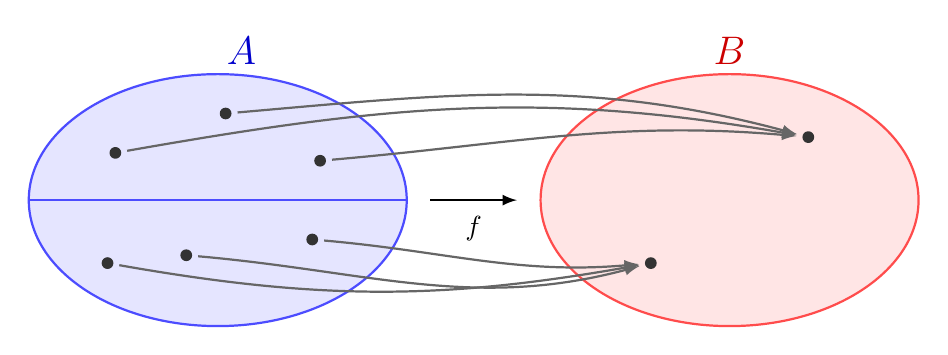
\begin{tikzpicture}[>=latex]

% --- Global TikZ Styles for Consistency ---
\tikzset{
    setA/.style={fill=blue!10, draw=blue!70, thick},
    setB/.style={fill=red!10, draw=red!70, thick},
    labelA/.style={text=blue!80!black, font=\Large\bfseries},
    labelB/.style={text=red!80!black, font=\Large\bfseries},
    point/.style={circle, fill=black!80, inner sep=1.5pt},
    arrow/.style={->, >=latex, thick, draw=black!60, shorten >=2pt, shorten <=2pt}
}

    % Verzameling A
    \path[setA] (0, 0) ellipse (2.4cm and 1.6cm);
    \node[labelA] at (0.3, 1.9) {$A$};
    
    % Horizontale scheidingslijn in A
    \draw[draw=blue!70, thick] (-2.4, 0) -- (2.4, 0);

    % Punten in bovenste helft van A
    \node[point] (a1) at (-1.3, 0.6) {};
    \node[point] (a2) at (0.1, 1.1) {};
    \node[point] (a3) at (1.3, 0.5) {};

    % Punten in onderste helft van A
    \node[point] (a4) at (-1.4, -0.8) {};
    \node[point] (a5) at (-0.4, -0.7) {};
    \node[point] (a6) at (1.2, -0.5) {};

    % Verzameling B
    \path[setB] (6.5, 0) ellipse (2.4cm and 1.6cm);
    \node[labelB] at (6.5, 1.9) {$B$};

    % Punten in B
    \node[point] (b1) at (7.5, 0.8) {};
    \node[point] (b2) at (5.5, -0.8) {};

    % Functiepijl en label f in het midden
    \draw[->, >=latex, thick] (2.7, 0) -- (3.8, 0) node[midway, below=2pt] {$f$};

    % Pijlen van A naar B (bovenste helft)
    % De "out" en "in" hoeken zorgen voor de vloeiende curves
    \draw[arrow] (a1) to[out=10, in=170] (b1);
    \draw[arrow] (a2) to[out=5, in=165] (b1);
    \draw[arrow] (a3) to[out=5, in=175] (b1);

    % Pijlen van A naar B (onderste helft)
    \draw[arrow] (a4) to[out=-10, in=190] (b2);
    \draw[arrow] (a5) to[out=-5, in=195] (b2);
    \draw[arrow] (a6) to[out=-5, in=185] (b2);
    
\end{tikzpicture}
}
\end{center}

\textbf{2.} Gegeven de equivalentierelatie $S$ voor $A$, dan is $c_S : A \to A/S$ een afbeelding: de canonieke afbeelding van de equivalentierelatie $S$.

\begin{center}
\resizebox{0.75\textwidth}{!}{%
    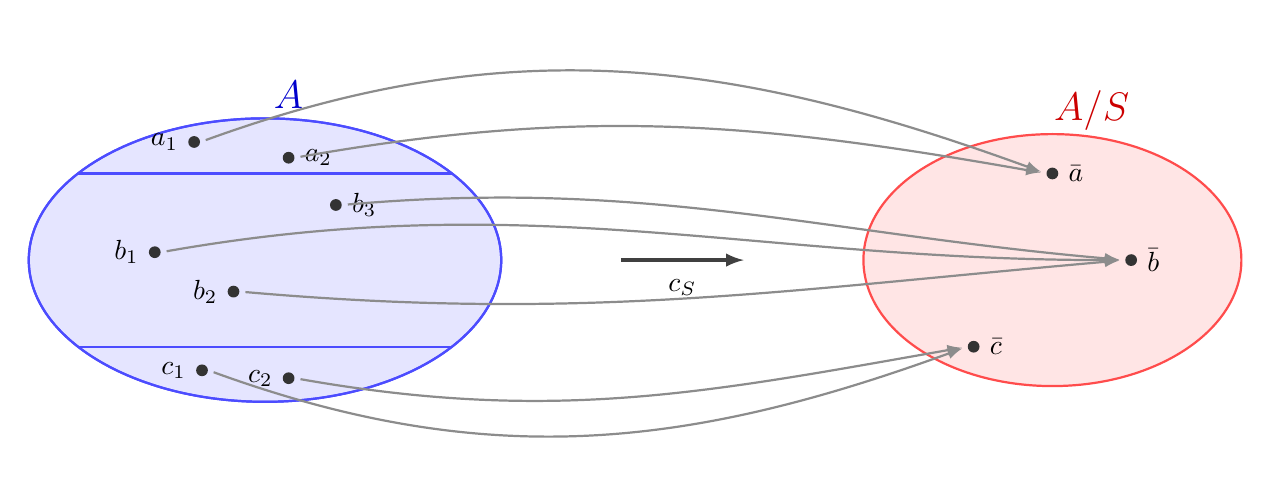
\begin{tikzpicture}[>=latex]

% --- Global TikZ Styles for Consistency ---
\tikzset{
    setA/.style={fill=blue!10, draw=blue!70, thick},
    setB/.style={fill=red!10, draw=red!70, thick},
    labelA/.style={text=blue!80!black, font=\Large\bfseries},
    labelB/.style={text=red!80!black, font=\Large\bfseries},
    partition/.style={draw=blue!70, thick},
    point/.style={circle, fill=black!80, inner sep=1.5pt},
    arrow/.style={
        ->,
        >=latex,
        thick,
        draw=black!45,
        shorten >=2pt,
        shorten <=2pt
    },
    mainarrow/.style={
        ->,
        >=latex,
        very thick,
        draw=black!75,
        shorten >=2pt,
        shorten <=2pt
    }
}

% Verzameling A
\path[setA] (0, 0) ellipse (3.0cm and 1.8cm);
\node[labelA] at (0.3, 2.1) {$A$};

% Partition Lines clipped inside A
\begin{scope}
    \clip (0, 0) ellipse (3.0cm and 1.8cm);
    \draw[partition] (-3.2, 1.1) -- (3.2, 1.1);
    \draw[partition] (-3.2, -1.1) -- (3.2, -1.1);
\end{scope}

% Redraw border of A so clipping does not visually affect the outline
\draw[blue!70, thick] (0, 0) ellipse (3.0cm and 1.8cm);

% Punten in A: top equivalence class
\node[point, label=left:$a_1$]  (at1) at (-0.9, 1.5) {};
\node[point, label=right:$a_2$] (at2) at (0.3, 1.3) {};
%\node[point, label=right:$a_3$] (at3) at (1.1, 1.5) {};

% Punten in A: middle equivalence class
\node[point, label=left:$b_1$]  (am1) at (-1.4, 0.1) {};
\node[point, label=left:$b_2$]  (am2) at (-0.4, -0.4) {};
\node[point, label=right:$b_3$] (am3) at (0.9, 0.7) {};
%\node[point, label=right:$b_4$] (am4) at (1.5, -0.1) {};

% Punten in A: bottom equivalence class
\node[point, label=left:$c_1$]  (ab1) at (-0.8, -1.4) {};
\node[point, label=left:$c_2$]  (ab2) at (0.3, -1.5) {};
%\node[point, label=right:$c_3$] (ab3) at (1.2, -1.4) {};

% Verzameling A/S
\path[setB] (10.0, 0) ellipse (2.4cm and 1.6cm);
\node[labelB] at (10.5, 1.9) {$A/S$};

% Punten in A/S
\node[point, label=right:$\bar{a}$] (bx) at (10.0, 1.1) {};
\node[point, label=right:$\bar{b}$] (by) at (11.0, 0.0) {};
\node[point, label=right:$\bar{c}$] (bz) at (9.0, -1.1) {};

% Canonical Quotient Mapping Arrow, centered between the two ellipses
% Right edge of A is x = 3.0, left edge of A/S is x = 7.6, midpoint is x = 5.3
\draw[mainarrow] (4.45, 0) -- (6.15, 0)
    node[midway, below=3pt] {$c_S$};

% Curved arrows from A to A/S: top class to X
\draw[arrow] (at1.east) to[out=20, in=160] (bx.west);
\draw[arrow] (at2.east) to[out=10, in=170] (bx.west);
%\draw[arrow] (at3.east) to[out=0,  in=180] (bx.west);

% Curved arrows from A to A/S: middle class to Y
\draw[arrow] (am1.east) to[out=10,  in=180] (by.west);
\draw[arrow] (am2.east) to[out=-5,  in=185] (by.west);
\draw[arrow] (am3.east) to[out=5,   in=175] (by.west);
%\draw[arrow] (am4.east) to[out=-10, in=190] (by.west);

% Curved arrows from A to A/S: bottom class to Z
\draw[arrow] (ab1.east) to[out=-20, in=200] (bz.west);
\draw[arrow] (ab2.east) to[out=-10, in=190] (bz.west);
%\draw[arrow] (ab3.east) to[out=0,   in=180] (bz.west);

\end{tikzpicture}
}
\end{center}

\textbf{3.} De vorige 2 kunnen we nu combineren:\newline
$\to$ De canonieke afbeelding $c_{R_f}$ van de equivalentierelatie $R_f$ gedefinieerd door de afbeelding $f$ noemt men de projectie van $f$ op $A/R_f$.

\begin{center}
\resizebox{0.65\textwidth}{!}{%
    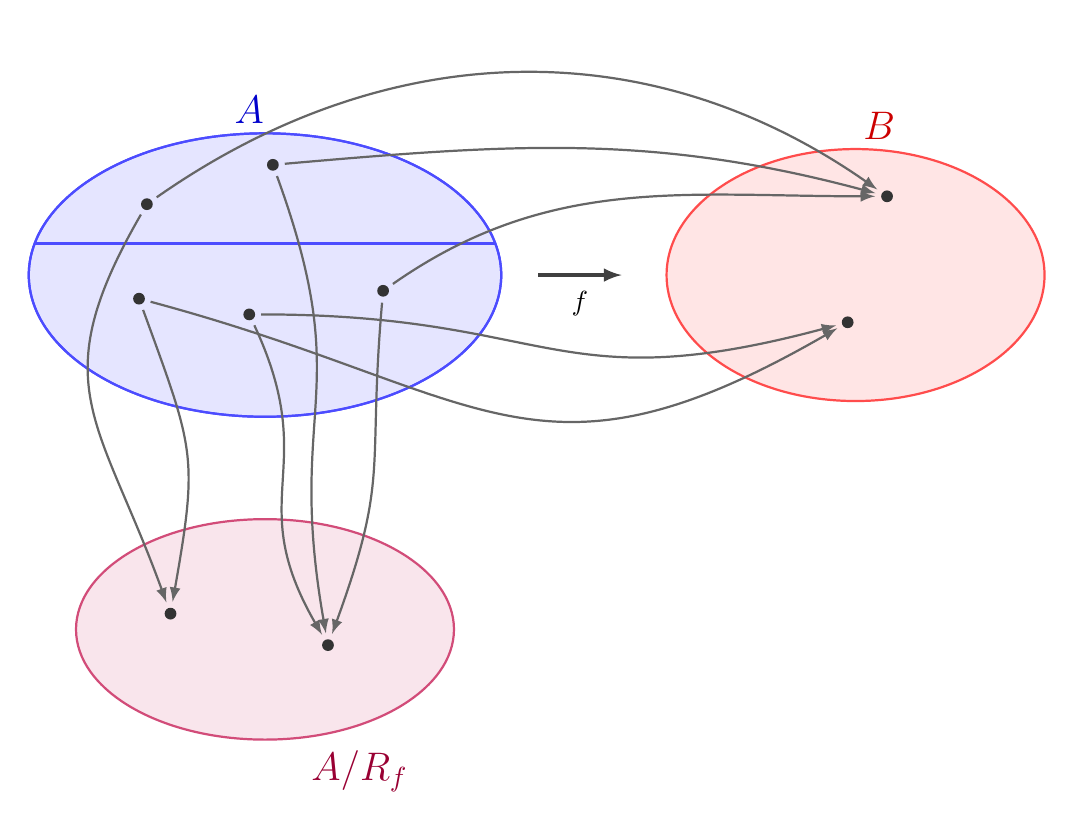
\begin{tikzpicture}[>=latex]

% --- Global TikZ Styles for Consistency ---
\tikzset{
    setA/.style={fill=blue!10, draw=blue!70, thick},
    setB/.style={fill=red!10, draw=red!70, thick},
    setC/.style={fill=purple!10, draw=purple!70, thick}, % Nieuwe stijl voor A/R_f
    labelA/.style={text=blue!80!black, font=\Large\bfseries},
    labelB/.style={text=red!80!black, font=\Large\bfseries},
    labelC/.style={text=purple!80!black, font=\Large\bfseries},
    partition/.style={draw=blue!70, thick},
    point/.style={circle, fill=black!80, inner sep=1.5pt},
    arrow/.style={
        ->,
        >=latex,
        thick,
        draw=black!60, % Iets donkerder gemaakt voor de vele overlappende lijnen
        shorten >=2pt,
        shorten <=2pt
    },
    mainarrow/.style={
        ->,
        >=latex,
        very thick,
        draw=black!75,
        shorten >=2pt,
        shorten <=2pt
    }
}

% --- Verzameling A (Boven Links) ---
\path[setA] (0, 0) ellipse (3.0cm and 1.8cm);
\node[labelA] at (-0.2, 2.1) {$A$};

% Partition Line clipped inside A
\begin{scope}
    \clip (0, 0) ellipse (3.0cm and 1.8cm);
    \draw[partition] (-3.2, 0.4) -- (3.2, 0.4);
\end{scope}

% Redraw border of A so clipping does not visually affect the outline
\draw[blue!70, thick] (0, 0) ellipse (3.0cm and 1.8cm);

% Punten in A
\node[point] (p1) at (-1.5, 0.9) {};  % linksboven
\node[point] (p2) at (0.1, 1.4) {};   % middenboven
\node[point] (p3) at (-1.6, -0.3) {}; % linksonder
\node[point] (p4) at (-0.2, -0.5) {}; % middenonder
\node[point] (p5) at (1.5, -0.2) {};  % rechtsonder

% --- Verzameling B (Boven Rechts) ---
% Iets hoger en naar rechts geplaatst zoals in de screenshot
\path[setB] (7.5, 0.0) ellipse (2.4cm and 1.6cm);
\node[labelB] at (7.8, 1.9) {$B$};

% Punten in B
\node[point] (b1) at (7.9, 1.0) {}; % Bovenste punt
\node[point] (b2) at (7.4, -0.6) {}; % Onderste punt

% --- Verzameling A/R_f (Onder Links) ---
\path[setC] (0, -4.5) ellipse (2.4cm and 1.4cm);
\node[labelC] at (1.2, -6.3) {$A/R_f$};

% Punten in A/R_f
\node[point] (q1) at (-1.2, -4.3) {}; % Linker punt
\node[point] (q2) at (0.8, -4.7) {};  % Rechter punt

% --- Pijlen en Mapping ---

% Hoofdpijl f (tussen A en B)
\draw[mainarrow] (3.4, 0.0) -- (4.6, 0.0) node[midway, below=2pt] {$f$};

% Pijlen van A naar B (Horizontale stroom)
\draw[arrow] (p1) to[out=35, in=145, looseness=1.0] (b1);
\draw[arrow] (p2) to[out=5,  in=165, looseness=1.0] (b1);
\draw[arrow] (p3) to[out=-15, in=210, looseness=1.3] (b2);
\draw[arrow] (p4) to[out=0,  in=195, looseness=1.3] (b2);
\draw[arrow] (p5) to[out=35, in=180] (b1); % Deze kronkelt mooi omhoog

% Pijlen van A naar A/R_f (Verticale stroom)
\draw[arrow] (p1) to[out=-120, in=110, looseness=1.3] (q1);
\draw[arrow] (p3) to[out=-70, in=80, looseness=1.3] (q1);
\draw[arrow] (p2) to[out=-70, in=100, looseness=1.3] (q2);
\draw[arrow] (p4) to[out=-65, in=120, looseness=1.3] (q2);
\draw[arrow] (p5) to[out=-95, in=70, looseness=1.3]  (q2);

\end{tikzpicture}
}
\end{center}

\begin{nicetheorem}*[ontbindingsstelling voor afbeeldingen]
    \nextpart[]*
    Iedere afbeelding $f:A \to B$ is te schrijven als een samenstelling
    \begin{equation}
        f = i \circ b \circ p \qedtag
    \end{equation}
    met
    \begin{itemize}
        \item $i = i_{\text{Ran }f}$ de inlassing van $\text{Ran }f = f(A)$ in $B$
        \item $b$ is een bijectie tussen $A/R_f = \text{Ran }p_f = p_f(A)$ en $f(A)$. Meer concreet; ze is gedefinieerd door $b(p_f(x)) = y \Leftrightarrow f(x) = y$
        \item $p = p_f$ is de projectie voor $f$ op $A/R_f$
    \end{itemize}
\end{nicetheorem}

\begin{center}
\resizebox{0.65\textwidth}{!}{%
    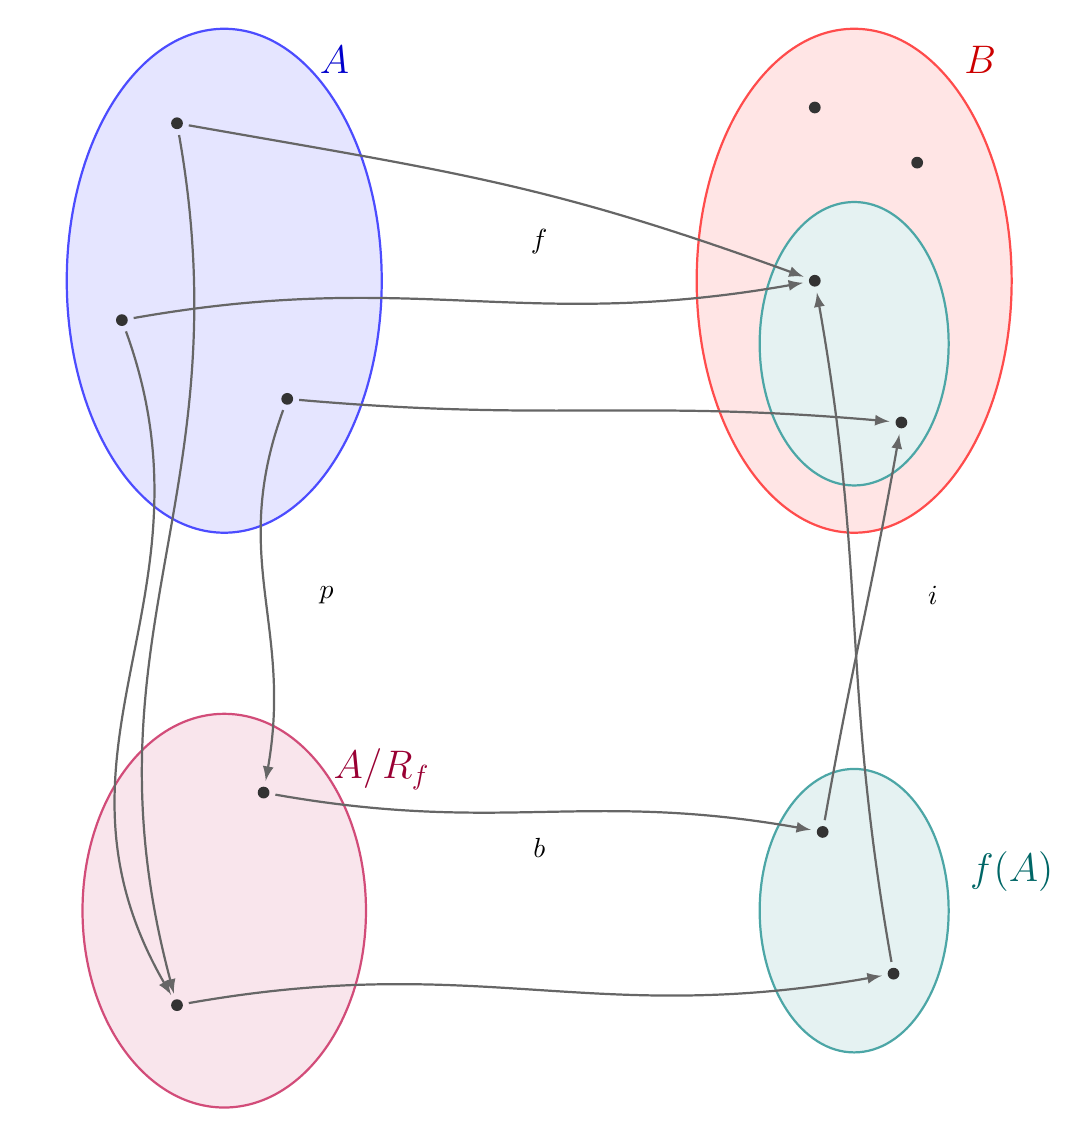
\begin{tikzpicture}[>=latex]

% --- Global TikZ Styles for Consistency ---
\tikzset{
    setA/.style={fill=blue!10, draw=blue!70, thick},
    setB/.style={fill=red!10, draw=red!70, thick},
    setC/.style={fill=purple!10, draw=purple!70, thick}, % Stijl voor A/R_f
    setD/.style={fill=teal!10, draw=teal!70, thick},     % Nieuwe stijl voor f(A)
    labelA/.style={text=blue!80!black, font=\Large\bfseries},
    labelB/.style={text=red!80!black, font=\Large\bfseries},
    labelC/.style={text=purple!80!black, font=\Large\bfseries},
    labelD/.style={text=teal!80!black, font=\Large\bfseries},
    point/.style={circle, fill=black!80, inner sep=1.5pt},
    arrow/.style={
        ->,
        >=latex,
        thick,
        draw=black!60, 
        shorten >=2pt,
        shorten <=2pt
    }
}

% --- Verzameling A (Boven Links) ---
\path[setA] (0, 4) ellipse (2.0cm and 3.2cm);
\node[labelA] at (1.4, 6.8) {$A$};

% Punten in A
\node[point] (p1) at (-0.6, 6.0) {};  % Boven
\node[point] (p2) at (-1.3, 3.5) {};  % Midden-links
\node[point] (p3) at (0.8, 2.5) {};   % Onder-rechts

% --- Verzameling B (Boven Rechts) ---
\path[setB] (8, 4) ellipse (2.0cm and 3.2cm);
\node[labelB] at (9.6, 6.8) {$B$};

% Inner f(A) subset in B (Teal gekleurd om te matchen met de set eronder)
\path[setD] (8, 3.2) ellipse (1.2cm and 1.8cm);

% Punten in B (Outer)
\node[point] (b3) at (7.5, 6.2) {};
\node[point] (b4) at (8.8, 5.5) {};

% Punten in B (Inner / f(A))
\node[point] (b1) at (7.5, 4.0) {};   % Bovenste in subset
\node[point] (b2) at (8.6, 2.2) {};   % Onderste in subset

% --- Verzameling A/R_f (Onder Links) ---
\path[setC] (0, -4) ellipse (1.8cm and 2.5cm);
\node[labelC] at (2.0, -2.2) {$A/R_f$};

% Punten in A/R_f
\node[point] (q1) at (0.5, -2.5) {};  % Bovenste punt
\node[point] (q2) at (-0.6, -5.2) {}; % Onderste punt

% --- Verzameling f(A) (Onder Rechts) ---
\path[setD] (8, -4) ellipse (1.2cm and 1.8cm);
\node[labelD] at (10.0, -3.5) {$f(A)$};

% Punten in f(A)
\node[point] (r1) at (7.6, -3.0) {};  % Bovenste punt
\node[point] (r2) at (8.5, -4.8) {};  % Onderste punt


% ==========================================
% --- Pijlen en Mapping ---
% ==========================================

% f: A -> B (Horizontaal boven)
\draw[arrow] (p1) to[out=-10, in=160, looseness=1.1] (b1);
\draw[arrow] (p2) to[out=10,  in=190, looseness=1.1] (b1);
\draw[arrow] (p3) to[out=-5,  in=175, looseness=1.1] (b2);
\node at (4, 4.5) {$f$};

% p: A -> A/R_f (Verticaal links, pijlen kruisen elkaar)
\draw[arrow] (p1) to[out=-80,  in=105,  looseness=1.1] (q2);
\draw[arrow] (p2) to[out=-70,  in=120, looseness=1.1] (q2);
\draw[arrow] (p3) to[out=-110, in=80,  looseness=1.1] (q1);
\node at (1.3, 0) {$p$};

% b: A/R_f -> f(A) (Horizontaal onder)
\draw[arrow] (q1) to[out=-10, in=170, looseness=1.1] (r1);
\draw[arrow] (q2) to[out=10,  in=190, looseness=1.1] (r2);
\node at (4, -3.2) {$b$};

% i: f(A) -> B (Verticaal rechts, pijlen kruisen elkaar elegant)
\draw[arrow] (r1) to[out=80,  in=-100, looseness=1.1] (b2);
\draw[arrow] (r2) to[out=100, in=-80,  looseness=1.1] (b1);
\node at (9.0, 0) {$i$};

\end{tikzpicture}
}
\end{center}

Dus elke afbeelding $f:A \to B$ is te schrijven als $f = i \circ b \circ p$ met:
\begin{itemize}
    \item $p =$ de \textbf{projectie} $A \to A/R_f : x \mapsto R_x$ (stuurt elk element naar zijn klasse)
    \item $b =$ een \textbf{bijectie} $A/R_f \to f(A) : R_x \mapsto f(x)$ (verbindt klassen met beelden)
    \item $i =$ de \textbf{inlassing} $f(A) \to B$ (vergeet dat we in $f(A)$ zaten en zie het als element van $B$)
\end{itemize}
Intuïtief doet elke afbeelding dus 3 dingen:
\begin{enumerate}
    \item Ze identificeert elementen die hetzelfde beeld krijgen (de projectie "collapsed" gelijksoortige elementen)
    \item Ze geeft elk verschillend "type" een uniek beeld (de bijectie)
    \item Ze plaatst dat beeld in het codomein $B$ (de inlassing)
\end{enumerate}

\begin{niceexample}*
    Beschouw de afbeelding $f : \mathbb{Z} \to \mathbb{Z} : n \mapsto n^2$.
    \nextpart[]*
    We analyseren de afbeelding $f$ volgens de ontbindingsstelling. $f$ definieert een equivalentierelatie want neem bijvoorbeeld $f(-3) = f(3) = 9$, dus $-3 \sim 3$.
    \begin{itemize}
        \item $R_f$ heeft equivalentieklassen $\bar{0}, \bar{1}, \bar{2}, \bar{3}, \dots$, waar elke equivalentieklasse bestaat uit de elementen $\{n, -n\}$ met $n \ge 0$. Dus $\mathbb{Z}/R_f = \{\bar{0}, \bar{1}, \bar{2}, \bar{3}, \dots\}$. We hebben hier $n \ge 0$ als representant gekozen want $\bar{3} = \overline{-3}$ zijn dezelfde equivalentieklasse.
        \item $p : \mathbb{Z} \to \mathbb{Z}/R_f$ "collapses" alle elementen met zelfde beeld samen. Hier dus: "collapses" $-n$ en $n$ samen.
        \item $b : \mathbb{Z}/R_f \to f(\mathbb{Z}) : \bar{n} \mapsto n^2$ met $f(\mathbb{Z}) = \{0, 1, 4, 9, 16, \dots\}$ geeft elke equivalentieklasse een uniek beeld $n^2$
        \item $i : f(\mathbb{Z}) \to \mathbb{Z}$ is gewoon "vergeet dat dit kwadraten zijn"
        \item Controle van de ontbinding, neem bv. $n= -3$:
        \begin{equation*}
            -3 \xlongrightarrow{p} \bar{3} \xlongrightarrow{b} 9 \xlongrightarrow{i} 9 = f(-3) \text{ \emoji{check-mark-button}}
        \end{equation*}
    \end{itemize}
\end{niceexample}

\subsection{Geordende Verzamelingen}

We schrijven $xRy$ meestal als $x \le y$ wanneer $R$ een orderelatie is (reflexief, anti-symmetrisch, transitief).

\textbf{Let op:} de notatie "$\le$" misleidt. "Is deler van" op $\mathbb{Z}$ is ook een orderelatie (we kunnen schrijven: $3 \le 12$ in de zin "3 deelt 12"), maar 5 en 7 zijn dan \textbf{niet vergelijkbaar} ($5 \nmid 7$) dus kan je niet schrijven $5 \le 7$.

\SimpleHeading{Partieel vs volledig (totaal) geordend}

\textbf{Volledig (totaal) geordend:} voor elke twee elementen geldt $x \le y$ of $y \le x$. Bijvoorbeeld $\mathbb{R}$ met de gewone "$\le$".

\textbf{Partieel geordend:} dat hoeft niet, sommige elementen zijn onvergelijkbaar. Bijvoorbeeld $\mathbb{N}$ met deelbaarheid, of $2^A$ met $\subseteq$.

\begin{niceexample}*
    \nextpart[]*
    \underline{Gegeven:} Beschouw de verzameling
    \begin{equation*}
        A = \{1,2,3\}
    \end{equation*}
    We bekijken nu de machtsverzameling van $A$:
    \begin{equation*}
        2^A = 2^{\{1,2,3\}}
    \end{equation*}
    Dit is de verzameling van alle deelverzamelingen van $A$:
    \begin{equation*}
        2^A = 
        \{\;
        \emptyset,
        \{1\},
        \{2\},
        \{3\},
        \{1,2\},
        \{1,3\},
        \{2,3\},
        \{1,2,3\}
        \;\}
    \end{equation*}
    Op $2^A$ bekijken we de relatie $\subseteq$, dus "is een deelverzameling van".

    \vspace{0.25cm}

    \underbar{Vraag:} Zijn de verzamelingen 
    \begin{equation*}
        \{1,2\} \qquad \text{en} \qquad \{2,3\}
    \end{equation*}
    vergelijkbaar voor de orde $\subseteq$? Met andere woorden: geldt één van de volgende 2 uitspraken?
    \begin{equation*}
        \{1,2\} \subseteq \{2,3\} \qquad \text{of} \qquad \{2,3\} \subseteq \{1,2\}
    \end{equation*}
    \underbar{Oplossing:} We controleren eerst of $\{1,2\} \subseteq \{2,3\}$ geldt. Dit zou betekenen dat elk element van $\{1,2\}$ ook een element is van $\{2,3\}$. Maar:
    \begin{equation*}
        1 \in \{1,2\} \qquad \text{en} \qquad 1 \notin \{2,3\}
    \end{equation*}
    Dus: $\{1,2\} \nsubseteq \{2,3\}$. (1)

    \vspace{0.25cm}

    We controleren nu omgekeerd of $\{2,3\} \subseteq \{1,2\}$ geldt. Dit zou betekenen dat elk element van $\{2,3\}$ ook een element is van $\{1,2\}$. Maar:
    \begin{equation*}
        3 \in \{2,3\} \qquad \text{en} \qquad 3 \notin \{1,2\}
    \end{equation*}
    Dus: $\{2,3\} \nsubseteq \{1,2\}$. (2)

    \vspace{0.25cm}

    Uit (1) en (2) volgt dan dat $\{1,2\}$ en $\{2,3\}$ niet vergelijkbaar zijn voor de orde $\subseteq$.

    \vspace{0.25cm}

    \underbar{Conclusie:} De relatie $\subseteq$ op $2^{\{1,2,3\}}$ is een partiële orde, maar geen totale orde. Ze is een partiële orde omdat $\subseteq$ reflexief, antisymmetrisch en transitief is. Ze is geen totale orde, omdat niet elk paar elementen vergelijkbaar is.
\end{niceexample}

\SimpleHeading{Bijzondere elementen voor een deelverzameling $B \subseteq A$}

\begin{center}
    \renewcommand{\arraystretch}{1.5}
    %\arrayrulecolor{gray!20}  % Change this to your desired color
    % \setlength{\arrayrulewidth}{1pt}  % Change this value (default is 0.4pt)
    \begin{tabularx}{\linewidth}{@{} >{\hsize=1.0\hsize}L >{\hsize=0.4\hsize}L >{\hsize=1.6\hsize}L @{}}
        \textbf{Begrip} & \textbf{Moet in $B$ zitten?} & \textbf{Wat is het?} \\
        \hline
        \textbf{Initieel element} van $B$ & Ja & Geen enkel ander element van $B$ gaat het strikt vooraf \\
        \thinrule
        \textbf{Terminaal element} van $B$ & Ja & Geen enkel ander element van $B$ komt er strikt na \\
        \thinrule
        \textbf{Ondergrens} van $B$ & Nee & Element van $A$ dat $\le$ is dan alle elementen van $B$ \\
        \thinrule
        \textbf{Bovengrens} van $B$ & Nee & Element van $A$ dat $\ge$ is dan alle elementen van $B$ \\
        \thinrule
        \textbf{Kleinste element} van $B$ & Ja & Ondergrens die in $B$ zelf zit \\
        \thinrule
        \textbf{Grootste element} van $B$ & Ja & Bovengrens die in $B$ zelf zit \\
        \thinrule
        \textbf{Infimum} van $B$ (grootste ondergrens) & Nee & Grootste van de ondergrenzen \\
        \thinrule
        \textbf{Supremum} van $B$ (kleinste bovengrens) & Nee & Kleinste van de bovengrenzen \\
        \hline
    \end{tabularx}
\end{center}

\begin{barbox}[red!66][red!1]
    \emoji{double-exclamation-mark} \textbf{Cruciaal onderscheid:} een kleinste element moet in $B$ zitten, een infimum niet.
\end{barbox}

\textbf{\underbar{Voorbeeld:}} In $\mathbb{R}$, beschouw $B = [0,1) \subset \mathbb{R}$
\begin{itemize}
    \item Kleinste element van $B$: 0 (zit in $B$ en is ondergrens)
    \item Grootste element van $B$: bestaat niet! (1 zit niet in $B$, en geen ander element is groter dan alle andere)
    \item Infimum van $B$: 0 (zelfde als kleinste, want het zit in $B$)
    \item Supremum van $B$: 1 (kleinste bovengrens, maar zit niet in $B$)
\end{itemize}

\subsubsection{Hasse-diagrammen}

Je kan een partieel geordende verzameling grafisch voorstellen door de pijlen van de relatie te tekenen. De pijlen die het gevolg zijn van transitiviteit en de lussen die het gevolg zijn van reflexiviteit laat je weg. 

\textbf{\underbar{Voorbeeld:}} Beschouw de verzameling $\{1,2,3,6\}$ met deelbaarheid. 

\noindent
\begin{minipage}[t]{0.55\textwidth}
\vspace{0pt} % Dwingt de absolute top-uitlijning af
\begin{itemize}
    \item 1 deelt alles $\to$ onderaan
    \item 2 deelt 6, 3 deelt 6 $\to$ 2 en 3 staan op gelijke hoogte boven 1, met lijn naar 6 erboven
\end{itemize}
\end{minipage}% <--- Dit procentteken is belangrijk om ongewenste witruimte te voorkomen!
\hfill
\begin{minipage}[t]{0.35\textwidth}
\vspace{0pt} % Zorgt dat de bovenkant van de figuur hier op gelijke hoogte start
\begin{center}
\resizebox{0.65\textwidth}{!}{%  % Schalen naar de breedte van deze minipage zelf
    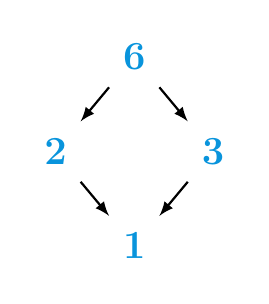
\begin{tikzpicture}[>=latex]

% --- Stijldefinities ---
\tikzset{
    getal/.style={
        text=cyan!80!blue, 
        font=\Large\bfseries, 
        inner sep=6pt
    },
    pijl/.style={
        ->,
        >=latex,
        thick,
        draw=black, % Past mooi bij de kleur van de getallen
        shorten >=0.1pt,      % Zorgt dat de pijl het getal niet snijdt
        shorten <=0.1pt
    }
}

% --- Knooppunten (Nodes) ---
\node[getal] (n6) at (0, 2.4) {6};
\node[getal] (n2) at (-1, 1.2) {2};
\node[getal] (n3) at (1, 1.2)  {3};
\node[getal] (n1) at (0, 0)   {1};

% --- Pijlen ---
\draw[pijl] (n6) -- (n3);
\draw[pijl] (n6) -- (n2);
\draw[pijl] (n2) -- (n1);
\draw[pijl] (n3) -- (n1);
\end{tikzpicture}
}
\end{center}
\end{minipage}

\textbf{\underbar{Voorbeeld:}} Beschouw een iets complexer voorbeeld. De deelbaarheidsrelatie voor de verzameling $\{2,4,8,64,40,12,6,30,60\}$.

$\to$ We gebruiken \Cref{alg:l3_hasse} om dit op te lossen.

\textbf{1.} Deelbare paren $(a \prec b)$:
\begin{equation*}
    \begin{gathered}
        2 \prec 4, \quad 2 \prec 8, \quad 2 \prec 64, \quad 2 \prec 40, \quad 2 \prec 12, \quad 2 \prec 6, \quad 2 \prec 30, \quad 2 \prec 60 \\[1ex]
        4 \prec 8, \quad 4 \prec 64, \quad 4 \prec 40, \quad 4 \prec 12, \quad 4 \prec 60 \\[1ex]
        8 \prec 64, \quad 8 \prec 40 \\[1ex]
        6 \prec 12, \quad 6 \prec 30, \quad 6 \prec 60 \\[1ex]
        12 \prec 60, \quad 30 \prec 60
    \end{gathered}
\end{equation*}

\textbf{2. + 3.} Verwijder transitieve paren:
\begin{itemize}
    \item $2 \prec 8$ want $2 \prec 4 \prec 8$
    \item $2 \prec 12$ want $2 \prec 4 \prec 12$ of $2 \prec 6 \prec 12$
    \item $2 \prec 60$ want $2 \prec 6 \prec 30 \prec 60$
    \item \dots
\end{itemize}

\textbf{4. + 5.}
\begin{center}
\resizebox{0.50\textwidth}{!}{%
    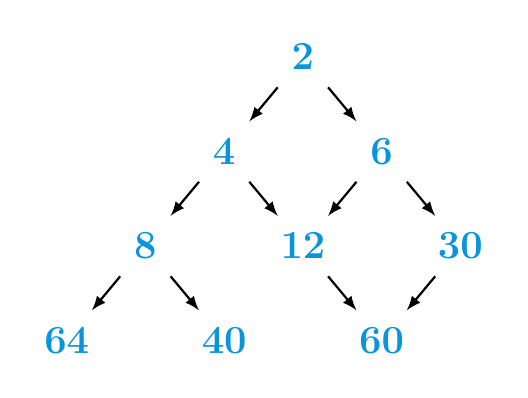
\begin{tikzpicture}[>=latex]

% --- Stijldefinities (gebaseerd op jouw aanpassingen) ---
\tikzset{
    getal/.style={
        text=cyan!80!blue, 
        font=\Large\bfseries, 
        inner sep=6pt
    },
    pijl/.style={
        ->,
        >=latex,
        thick,
        draw=black, 
        shorten >=0.1pt,      
        shorten <=0.1pt
    }
}

% --- Knooppunten (Nodes) ---

% Niveau 0 (Top)
\node[getal] (n2) at (0, 3.6) {2};

% Niveau 1
\node[getal] (n4) at (-1, 2.4) {4};
\node[getal] (n6) at (1, 2.4)  {6};

% Niveau 2
\node[getal] (n8)  at (-2, 1.2) {8};
\node[getal] (n12) at (0, 1.2)  {12};
\node[getal] (n30) at (2, 1.2)  {30};

% Niveau 3 (Bottom)
\node[getal] (n64) at (-3, 0) {64};
\node[getal] (n40) at (-1, 0) {40};
\node[getal] (n60) at (1, 0)  {60};


% --- Pijlen (van boven naar beneden) ---

% Verbindingen vanaf 2
\draw[pijl] (n2) -- (n4);
\draw[pijl] (n2) -- (n6);

% Verbindingen vanaf 4 en 6
\draw[pijl] (n4) -- (n8);
\draw[pijl] (n4) -- (n12);
\draw[pijl] (n6) -- (n12);
\draw[pijl] (n6) -- (n30);

% Verbindingen vanaf 8, 12 en 30
\draw[pijl] (n8) -- (n64);
\draw[pijl] (n8) -- (n40);
\draw[pijl] (n12) -- (n60);
\draw[pijl] (n30) -- (n60);

\end{tikzpicture}
}
\end{center}

Uit dit Hasse diagram kan je nu gemakkelijk dingen aflezen:
\begin{itemize}
    \item 2 is het kleinste element, er is geen grootste element.
    \item 2 is een initieel element
    \item 64, 40 en 64 zijn terminale elementen.
    \item 2, 4, 6 en 12 zijn ondergrenzen voor de deelverzameling $\{12, 60\}$. Deze verzameling ondergrenzen heeft een grootste element nl. 12. 12 is daarom het infimum van de deelverzameling $\{12, 60\}$.
    \item $\{12, 60\}$ heeft slechts 1 bovengrens nl. 60. Dit is tegelijk het grootste element en het supremum van $\{12, 60\}$. (Er moet gelden $12 \mid x$ en $60 \mid x$ dus niet 64 maar 60 als bovengrens!)
\end{itemize}

\begin{nicealgorithm}*[Hasse-diagram]\label{alg:l3_hasse}
    Een algemeen algoritme om een Hasse-diagram te maken.
    \nextpart[Algoritme.]*
    Gegeven een verzameling $A$ en een relatie $R$ zodat $A$ een partieel geordende verzameling is voor de relatie $R$:
    \begin{enumerate}
        \item Vindt alle paren $(a,b)$ waar $aRb$ en $a \neq b$.
        \item Voor elk paar $(a,b)$, controleer als er een $c \in A$ bestaat zodat
        \begin{equation*}
            aRc \quad \text{en} \quad cRb \qquad \text{ met } \quad c \neq a,b \qquad \text{(transitiviteit)}
        \end{equation*}
        \item Als zo een $c$ bestaat, verwijder dan $(a,b)$.
        \item De paren die overblijven zijn de \emph{edges} van het Hasse diagram.
        \item Teken van boven naar onder, geordend.
    \end{enumerate}
\end{nicealgorithm}

\subsection{Recursiviteit}

\emoji{pushpin} \inlinecode{TODO}[red!22] \emoji{pushpin} 

\subsection{Tellen en meten}

\begin{nicedefinition}*[Equipotentie]
    \nextpart[]*
    Twee verzamelingen zijn \textcolor{PineGreen!75!black}{\textbf{equipotent}} indien er een bijectie tussen hen bestaat. Intuïtief: ze hebben "evenveel" elementen.
\end{nicedefinition}

\textbf{\underbar{Voorbeeld:}}
\begin{itemize}
    \item $\mathbb{N}$ en de even getallen zijn equipotent ($n \mapsto 2n$ is een bijectie).
    \item $\mathbb{N} \text{ en } \mathbb{Q}$ zijn equipotent. (zie diagonaalargument in de cursustekst: rangschik breuken eerst op "teller+noemer" som en dan map elk natuurlijk getal naar een rationaal getal uit deze oneindige rij)
    \item $\mathbb{N}$ en $\mathbb{R}$ zijn niet equipotent (Cantor) (Je kan de reële getallen niet op een rij zetten, je kan er steeds eentje tussen blijven steken)
\end{itemize}

\begin{nicenote}*
    Waarom zijn $\mathbb{N}$ en de even getallen een bijectie? Heeft $\mathbb{N}$ niet dubbel zoveel getallen?
    \nextpart[]*
    Dit voelt tegenintuïtief. Bij \textbf{eindige} verzamelingen klopt dit:
    \begin{equation*}
        \{1,2,3,4,5,6\}
    \end{equation*}
    heeft dubbel zoveel elementen als
    \begin{equation*}
        \{2,4,6\}
    \end{equation*}
    Maar bij \textbf{oneindige} verzamelingen werkt "dubbel zoveel" anders. Daar kijk je niet naar dichtheid of verhouding, maar naar: "\textbf{kunnen we elk element van de ene verzameling precies koppelen aan één element van de andere?}"

    \vspace{0.25cm}

    Voor $\mathbb{N}$ en de even getallen kan dat:
    \begin{equation*}
        f(n) = 2n
    \end{equation*}
    Bijvoorbeeld, als $\mathbb{N} = \{1,2,3,4,\dots\}$, dan:
    \begin{equation*}
        \begin{aligned}
            1 &\mapsto 2 \\
            2 &\mapsto 4 \\
            3 &\mapsto 6 \\
            4 &\mapsto 8 
        \end{aligned}
    \end{equation*}
    enzovoort. Elke natuurlijk getal krijgt precies één getal, en elk even getal komt precies één keer voor.
\end{nicenote}

\begin{nicedefinition}*[Aftelbaarheid]
    \nextpart[]*
    $A$ is \textcolor{PineGreen!75!black}{\textbf{aftelbaar}} als er een bijectie bestaat met $\mathbb{N}$ of een eindig deel ervan.

    \vspace{0.25cm}

    Als er een bijectie bestaat tussen de verzameling $A$ en $\{1,2,\dots,m\}$, dan zegt men dat $A$ $m$ elementen heeft.
\end{nicedefinition}

\begin{nicedefinition}*[Cardinaliteit]
    \nextpart[]*
    $\#A$ = aantal elemten van $A$. Deze functie voldoet aan de volgende eigenschappen:
    \begin{itemize}
        \item $\#\emptyset = 0$
        \item $A \cap B = \varnothing \quad \Rightarrow \quad \#(A \cup B) = \#A + \#B$
        \item $\#(2^A) = 2^{\#A}$
    \end{itemize}
\end{nicedefinition}

\subsection{Samenstellingswetten}

Dit is de brug naar de algebra. We gaan elementen "combineren".

\begin{nicedefinition}*\label{def:inwendige_samenstellingswet}
    \nextpart[]*
    Een \textcolor{PineGreen!75!black}{\textbf{inwendige samenstellingswet}} of \textcolor{PineGreen!75!black}{\textbf{bewerking}} onder de elementen van $A$ is een afbeelding van $B \subseteq A \times A \to A:$
    \begin{equation*}
        (x,y) \mapsto z = f((x,y))
    \end{equation*}
    Ze combineert dus 2 elementen van $A$ tot één element van $A$.

    \vspace{0.25cm}

    Notatie:
    \begin{itemize}
        \item $x \top y$ (algemeen)
        \item $x + y$ (additief)
        \item $x \cdot y$ of $xy$ (multiplicatief)
    \end{itemize}
    De verzameling $A$ die voorzien is van de bewerking $\top$ noteren we als $\langle A, \top \rangle$.
\end{nicedefinition}

\begin{niceproperty}*
    Eigenschappen die een wet $\top$ kan hebben
    \nextpart[]*
    \begin{center}
        \renewcommand{\arraystretch}{1.5}
        \arrayrulecolor{gray!20}
        \setlength{\arrayrulewidth}{1pt}
        \begin{tabularx}{\linewidth}{@{} | >{\hsize=0.6\hsize}L | >{\hsize=1.4\hsize}L | @{}}
            \hline
            \cellcolor{RoyalPurple!75!black}\textcolor{white}{\textbf{Eigenschap}} & \cellcolor{RoyalPurple!75!black}\textcolor{white}{\textbf{Definitie}} \\
            \hline
            \cellcolor{RoyalPurple!5} Overal bepaald & $\top$ gedefinieerd voor alle $(x,y) \in A \times A$ \\
            \hline
            \cellcolor{RoyalPurple!5} Associatief & $x \top (y \top z) = (x \top y) \top z$ \\
            \hline
            \cellcolor{RoyalPurple!5} Commutatief & $x \top y = y \top x$ \\
            \hline
            \cellcolor{RoyalPurple!5} Neutraal element $e$ & $x \top e = e \top x = x$ voor alle $x$ \\
            \hline
            \cellcolor{RoyalPurple!5} $E \subseteq A$ is \textbf{stabiel} voor $\top$ & $x, y \in E \Rightarrow x \top y \in E$ \\
            \hline
        \end{tabularx}
    \end{center}
\end{niceproperty}

\begin{nicetheorem}*
    Als een neutraal element bestaat is het \textcolor{red!75!black}{\textbf{uniek}}!
    \nextpart[Bewijs.]*
    Stel dat $e_1$ en $e_2$ beide neutrale elementen zijn, dan is, omdat $e_1$ een neutraal element is
    \begin{equation*}
        e_2 \top e_1 = e_1 \top e_2 = e_2
    \end{equation*}
    en omdat $e_2$ een neutraal element is
    \begin{equation*}
        e_1 \top e_2 = e_2 \top e_1 = e_1
    \end{equation*}
    Vanwege het 1-waardig zijn is dus $e_1 = e_2$.
\end{nicetheorem}

\SimpleHeading{Regulariteit en Symmetriseerbaarheid}

\begin{nicedefinition}*
    \nextpart[]*
    $l \in A$ heet \textcolor{PineGreen!75!black}{\textbf{links-regulier}} voor $\top$ \emph{asa}
    \begin{equation}
        l \top x = l \top y \Rightarrow x = y, \qquad \forall x, y \in A \qedtag
    \end{equation}
    Dit wil zeggen dat $x \mapsto l \top x$ een \textbf{injectie} is. Het schrappen van $l$ is een linker inverse afbeelding voor deze injectie.

    \vspace{0.5cm}

    $r \in A$ heet \textcolor{PineGreen!75!black}{\textbf{rechts-regulier}} voor $\top$ \emph{asa}
    \begin{equation}
        x \top r = t \top r \Rightarrow x = y, \qquad \forall x, y \in A \qedtag
    \end{equation}
    Dit wil zeggen dat $x \mapsto x \top r$ een injectie is. Het schrappen van $r$ is een \textbf{\underbar{linker}} inverse afbeelding voor deze injectie.

    \vspace{0.5cm}

    Een element heet regulier als het zowel links- als rechts-regulier is.
\end{nicedefinition}

\begin{nicedefinition}*
    \nextpart[]*
    Zij $e$ het neutraal element van $\langle A, \top \rangle$, dan is $x\in A$ symmetriseerbaar voor $\top$ \emph{asa}
    \begin{equation}
        \exists y \in A \qquad \text{zodat} \qquad x \top y = e \quad \text{en} \quad y \top x = e
    \end{equation}
    $y$ heet dan het symmetrische element van $x$ voor $\top$. Notatie: $y = sym(x)$.
\end{nicedefinition}

\begin{nicetheorem}*
    \nextpart[]*
    Als $\top$ associatief is, dan is
    \begin{enumerate}
        \item $sym(x)$ is uniek (het symmetrische element van $x \in A$ is enig)
        \item Symmetriseerbare elementen zijn regulier
        \item $sym(x \top y) = sym(y) \;\top\; sym(x)$ (\textcolor{red!75!black}{\textbf{Let op de volgorde!}})
    \end{enumerate}
\end{nicetheorem}

\textbf{\underbar{Notatie:}}
\begin{center}
    \renewcommand{\arraystretch}{1.5}
    \arrayrulecolor{black}
    %\setlength{\arrayrulewidth}{1pt}
    \begin{tabularx}{\linewidth}{@{} >{\hsize=1.8\hsize}L >{\hsize=0.7\hsize}C >{\hsize=0.5\hsize}C >{\hsize=0.5\hsize}C >{\hsize=0.5\hsize}C @{}}
        \textbf{Soort wet} & \textbf{Bewerking} & \textbf{Neutraal} & \textbf{Sym$(x)$} & \textbf{Iteratie} \\
        \hline
        \textbf{Additief} (associatief + commutatief) & $x+y$ & 0 & $-x$ & $nx$ \\
        \thinrule
        \textbf{Multiplicatief} (associatief, niet noodzakelijk commutatief) & $xy$ & 1 & $x^{-1}$ & $x^n$ \\
        \hline
    \end{tabularx}
\end{center}

\SimpleHeading{Distrubitiviteit}

$\top_1$ is links-distrubitief over $\top_2$: $\quad x\; \top_1\; (y\; \top_2\; z) = (x\; \top_1\; y)\; \top_2\; (x\; \top_1\; z)$

\textbf{\underbar{Voorbeeld:}} In $\mathbb{R}$ is \inlinetext{$\cdot$} links-distrubitief over \inlinetext{$+$}: $\quad x(y+z) = xy + xz$

\SimpleHeading{Uitwendinge samenstellingswet}

Herinner \Cref{def:inwendige_samenstellingswet}: een \textbf{inwendige samenstellingswet} op een verzameling $A$ is een bewerking die 2 elementen van $A$ neemt en opnieuw een element van $A$ geeft.
\begin{equation*}
    \top : A \times A \to A
\end{equation*}
of concreet:
\begin{equation*}
    (x,y) \mapsto x\; \top\; y
\end{equation*}
\textbf{\underbar{Voorbeelden:}} 2 inwendige samenstellingswetten op $\mathbb{R}$:
\begin{itemize}
    \item 2 reële getallen optellen geeft opnieuw een reëel getal:
    \begin{equation*}
        + : \mathbb{R} \times \mathbb{R} \to \mathbb{R}
    \end{equation*}
    \item 2 reële getallen vermenigvuldigen geeft opnieuw een reëel getal:
    \begin{equation*}
        \cdot : \mathbb{R} \times \mathbb{R} \to \mathbb{R}
    \end{equation*}
\end{itemize}

\begin{nicedefinition}*{Uitwendinge Samenstellingswet}
    \nextpart[]*
    Een \textcolor{PineGreen!75!black}{\textbf{Uitwendinge samenstellingswet}} combineert één element uit een andere verzameling $\Omega$ met één element uit $A$.
    \begin{equation*}
        \begin{gathered}
            \Omega \times A \to A \\
            (\alpha, x) \mapsto \alpha \perp x
        \end{gathered}
    \end{equation*}
    $\Omega$ noemt men het \textbf{operatorengebied}: de verzameling van dingen die "werken op" elementen van $A$.
\end{nicedefinition}

\textbf{\underbar{Voorbeeld:}} Neem
\begin{equation*}
    \Omega = \mathbb{R} \qquad \text{en} \qquad A = \mathbb{R}^2
\end{equation*}
Dan is:
\begin{equation*}
    \begin{gathered}
        \mathbb{R} \times \mathbb{R}^2 \to \mathbb{R}^2 \\
        (\alpha, (x,y)) \mapsto \alpha \cdot (x,y) = (\alpha x, \alpha y)
    \end{gathered}
\end{equation*}
Bijvoorbeeld:
\begin{equation*}
    3 \cdot (2,5) = (6, 15)
\end{equation*}
Hier combineer je dus $3 \in \mathbb{R}$ met $(2,5) \in \mathbb{R}^2$ en het resultaat is opnieuw een element uit $\mathbb{R}^2$.

\subsubsection{Verenigbaarheid en Quotiëntwetten}

Dit is een belangrijk stuk. Stel dat je een equivalentierelatie $R$ hebt op een verzameling $A$. Dan deelt $R$ de verzameling $A$ op in equivalentieklassen. (\Cref{theorem:ER_naar_E_klassen}).

Je wilt soms een bewerking $\top$ op $A$ gebruiken om een nieuwe bewerking op de equivalentieklassen te definieëren. Dus als je equivalentieklassen hebt:
\begin{equation*}
    \bar{x} \qquad \text{en} \qquad \bar{y},
\end{equation*}
dan wil je zeggen:
\begin{equationbox}[NavyBlue]
    \bar{x} \overline{\top} \bar{y} = \overline{x \top y}
\end{equationbox}
Maar dit mag alleen als het resultaat \inlinetext{niet afhangt van de gekozen representanten!}[Goldenrod!55]

Want $\bar{x}$ en $\bar{y}$ kunnen meerdere representanten hebben. Stel je neemt
\begin{equation*}
    x'\in \bar{x} \qquad \text{en} \qquad y' \in \bar{y},
\end{equation*}
dan geldt automatisch:
\begin{equation*}
    \bar{x} = \bar{x}' \qquad \text{en} \qquad \bar{y} = \bar{y}'
\end{equation*}
Dan zou je ook kunnen rekenen met $x'$ en $y'$:
\begin{equation*}
    \overline{x'\;\top\;y'}
\end{equation*}
Opdat de bewerking op equivalentieklassen goed gedefinieerd is, moet je altijd hetvolgende resultaat krijgen:
\begin{equation*}
    \overline{x\;\top\;y} = \overline{x'\;\top\;y'}
\end{equation*}
Dit is wat \inlinetext{verenigbaarheid}[Goldenrod!55] garandeert.

\SimpleHeading{Rechts-verenigbaar}

\begin{nicedefinition}*[Rechts-verenigbaar]
    \nextpart[]*
    Zij $A$ een verzameling met inwendige samenstellingswet $\top$ en een equivalentierelatie $R$. Dan is $R$ \textcolor{PineGreen!75!black}{\textbf{rechts-verenigbaar}} met $\top$ als
    \begin{equation*}
        xRy \Rightarrow (x\;\top\;a)\;R\;(y\;\top\;a), \qquad \forall a \in A
    \end{equation*}
    In woorden: als $x$ en $y$ verenigbaar zijn, dan blijven ze equivalent wanneer je an de rechterkant met hetzelfde element $a$ combineert.
\end{nicedefinition}

Dus: 
\begin{equation*}
    x \sim y
\end{equation*}
impliceert:
\begin{equation*}
    x\;\top\;a \;\sim\; y\;\top\;a
\end{equation*}
\textbf{\underbar{Voorbeeld:}} Als 
\begin{equation*}
    x \equiv y \quad \text{mod } m
\end{equation*}
dan geldt ook:
\begin{equation*}
    x+a \equiv y+a \quad \text{mod } m
\end{equation*}
Dit noem je rechts-verenigbaarheid van \inlinetext{congruentie modulo $m$} met optelling.

\SimpleHeading{Links-verenigbaar}

Analoog geldt dan:
\begin{nicedefinition}*[Links-verenigbaar]
    \nextpart[]*
    Zij $A$ een verzameling met inwendige samenstellingswet $\top$ en een equivalentierelatie $R$. Dan is $R$ \textcolor{PineGreen!75!black}{\textbf{links-verenigbaar}} met $\top$ als
    \begin{equation*}
        xRy \Rightarrow (a\;\top\;x) \;R\; (a\;\top\;y), \qquad \forall a \in A
    \end{equation*}
    In woorden: als $x$ en $y$ equivalent zijn, dan blijven ze equivalent wanneer je aan de linkerkant met hetzelfde element $a$ combineert.
\end{nicedefinition}

\textbf{\underbar{Voorbeeld:}} Bij optelling modulo $m$:
\begin{equation*}
    x \equiv y \quad \text{mod } m \Rightarrow a + x \equiv a + y \quad \text{mod } m
\end{equation*}

\SimpleHeading{Quotiëntwet}

\begin{nicetheorem}*[Quotiëntwet]\label{theo:H2_quotientwet}
    \nextpart[]*
    Zij $A$ een verzameling, $\top$ een inwendige samenstellingswet voor $A$ en $R$ een equivalentierelatie voor $A$ die verenigbaar is met $\top$, dan is $\overline{\top}$ gedefinieerd in de quotiëntverzameling $A/R$ als
    \begin{equation*}
        \overline{\top} : A/R \times A/R \to A/R : (\bar{x}, \bar{y}) \mapsto \bar{x}\;\overline{\top}\;\bar{y} = \overline{x\;\top\;y}
    \end{equation*}
    een inwendige samenstellingswet voor $A/R$.
\end{nicetheorem}

De quotiëntverzameling is de verzameling van alle equivalentieklassen:
\begin{equation*}
    A/R = \{\bar{x} \mid x \in A\}
\end{equation*}
De nieuwe bewerking op equivalentieklassen wordt:
\begin{equation*}
    \bar{x}\;\overline{\top}\; \bar{y} = \overline{x\;\top\;y}
\end{equation*}
Of zoals in de cursustekst genoteerd:
\begin{equation*}
    R_x \;\overline{\top}\; R_y = R_{x \top y}
\end{equation*}

\begin{barbox}[SeaGreen][gray!5]
    \textcolor{SeaGreen}{\textbf{Merk op:}} Je kan rekenen met representanten en de keuze van de representanten maakt niet uit!
\end{barbox}

\SimpleHeading{Motivatie: waarom is dit belangrijk}

Omdat een klasse meerdere representanten heeft. Neem bijvoorbeeld modulo 5:
\begin{equation*}
    \bar{2} = \{\dots, -3, 2, 7, 12, \dots\}
\end{equation*}
Dus $\bar{2}$ kan worden voorgesteld door 2, maar ook door 7, 12, -3, enzovoort. Als je nu wil definiëren:
\begin{equation*}
    \bar{2} + \bar{3} = \overline{2+3} = \bar{5} = \bar{0}
\end{equation*}
dan moet dit hetzelfde resultaat geven als je andere representanten kiest. Bijvoorbeeld:
\begin{equation*}
    7 \in \bar{2} \qquad \text{en} \qquad 8 \in \bar{3}
\end{equation*}
Dan:
\begin{equation*}
    7+8=15 \qquad \text{en} \qquad \bar{15} = 0
\end{equation*}
Dus inderdaad:
\begin{equation*}
    \overline{2+3} = \overline{7+8}
\end{equation*}
$\longrightarrow$ optellen modulo 5 is dus goed gedefinieerd op equivalentieklassen.

\textbf{\underbar{Voorbeeld: rekenen modulo $m$}}\newline
Neem de equivalentierelatie:
\begin{equation*}
    a \sim b \Leftrightarrow a \equiv b \text{ mod } m
\end{equation*}
De equivalentieklassen zijn:
\begin{equation*}
    \bar{0}, \bar{1}, \bar{2}, \dots, \overline{m-1}
\end{equation*}
Definieër nu de optelling op deze equivalentieklassen door:
\begin{equation*}
    \bar{a} + \bar{b} = \overline{a + b}
\end{equation*}
Dit mag omdat we net hebben gezien dat volgens \Cref{theo:H2_quotientwet}, als $\top$ een inwendige samenstellingswet voor $A$ is en $R$ een equivalentierelatie voor $A$ die verenigbaar baar is met $\top$, dan is $\overline{\top}$ gedefinieerd in de quotiëntverzameling $A/R$ en is dit een inwendige samenstellingswet voor $A/R$.

Bijvoorbeeld modulo 5:
\begin{equation*}
    \bar{3} + \bar{4} = \overline{3+4} = \bar{7} = \bar{2}
\end{equation*}
Dit mag, want congruentie modulo $m$ is verenigbaar met optelling.

Ook vermenigvuldiging werkt:
\begin{equation*}
    \bar{a} \cdot \bar{b} = \overline{ab}
\end{equation*}
Bijvoorbeeld modulo 5:
\begin{equation*}
    \bar{3} \cdot \bar{4} = \bar{12} = \bar{2}
\end{equation*}
Ook dit is goed gedefinieerd, want congruentie modulo $m$ is verenigbaar met vermenigvuldiging.

\textbf{\underbar{Voorbeeld:}} Gegeven het volgende stelsel:
\begin{equation*}
\left\{
\begin{array}{rcrcrcl}
    2x_1 & - & 2x_2 & + & 3x_3 & = & 7 \pmod{5} \\
     x_1 & + &  x_2 &   &      & = & 3 \pmod{5} \\
    2x_1 & - &  x_2 & + & 2x_3 & = & 1 \pmod{5}
\end{array}
\right.
\end{equation*}
We lossen het op in $\mathbb{Z_5}$:
\begin{equation*}
\left\{
\begin{array}{rcrcrcl}
    \bar{2}\bar{x}_1 & - & \bar{2}\bar{x}_2 & + & \bar{3}\bar{x}_3 & = & \bar{2} \\
     \bar{x}_1 & + &  \bar{x}_2 &   &            & = & \bar{3} \\
    \bar{2}\bar{x}_1 & - &  \bar{x}_2 & + & \bar{2}\bar{x}_3 & = & \bar{1}
\end{array}
\right.
\end{equation*}
Doe Gauss-eliminatie. Mer op dat je \textbf{niet kan delen}. Vermenigvuldig (1) met 3:
\begin{equation*}
\left\{
\begin{array}{rcrcrcl}
     \bar{x}_1 & - &  \bar{x}_2 & +  & \bar{4}\bar{x}_3 & = & \bar{1} \\
     \bar{x}_1 & + &  \bar{x}_2 &    &            & = & \bar{3} \\
    \bar{2}\bar{x}_1 & - &  \bar{x}_2 & +  & \bar{2}\bar{x}_3 & = & \bar{1}
\end{array}
\right.
\xLongrightarrow[(3) + \bar{3}(1)]{(2) + \bar{4}(1)}
\left\{
\begin{array}{rcrcrcl}
     \bar{x}_1 & - & \bar{x}_2 & + & 4\bar{x}_3 & = & \bar{1} \\
               & - & \bar{3}\bar{x}_2 & + & \bar{x}_3 & = & \bar{2} \\
               & - & \bar{4}\bar{x}_2 & + & \bar{4}\bar{x}_3 & = & \bar{4}
\end{array}
\right.
\end{equation*}
Vermenigvuldig (2) met $\bar{2}$:
\begin{equation*}
\left\{
\begin{array}{rcrcrcl}
     \bar{x}_1 & - & \bar{x}_2 & + & 4\bar{x}_3 & = & \bar{1} \\
               & - & \bar{x}_2 & + & \bar{2}\bar{x}_3 & = & \bar{4} \\
               & - & \bar{4}\bar{x}_2 & + & \bar{4}\bar{x}_3 & = & \bar{4}
\end{array}
\right.
\xLongrightarrow{(3) + (2)}
\left\{
\begin{array}{rcrcrcl}
     \bar{x}_1 & - & \bar{x}_2 & + & 4\bar{x}_3       & = & \bar{1} \\
               & - & \bar{x}_2 & + & \bar{2}\bar{x}_3 & = & \bar{4} \\
               &   &           &   & \bar{x}_3        & = & \bar{3}
\end{array}
\right.  
\end{equation*}
Dan vind je:
\begin{equation*}
    x_3 = 3 \pmod{5}, \qquad x_2 = 2 \pmod{5}, \qquad x_1 = 1 \pmod{5}     
\end{equation*}

\begin{barbox}[red!66][red!1]
    \emoji{double-exclamation-mark} \textbf{Merk op:} $m$ is hier een priemgetal
\end{barbox}

Laten we nu eens hetzelfde doen voor $\mathbb{Z}_6$:

\textbf{\underbar{Voorbeeld:}} Gegeven het volgende stelsel:
\begin{equation*}
\left\{
\begin{array}{rcrcrcl}
    2x_1 & - & 2x_2 & + & 3x_3 & = & 7 \pmod{6} \\
     x_1 & + &  x_2 &   &      & = & 3 \pmod{6} \\
    2x_1 & - &  x_2 & + & 2x_3 & = & 1 \pmod{6}
\end{array}
\right.
\end{equation*}
We lossen het op in $\mathbb{Z_6}$:
\begin{equation*}
\left\{
\begin{array}{rcrcrcl}
    \bar{2}\bar{x}_1 & - & \bar{2}\bar{x}_2 & + & \bar{3}\bar{x}_3 & = & \bar{1} \\
     \bar{x}_1       & + & \bar{x}_2 &      &            & = & \bar{3} \\
    \bar{2}\bar{x}_1 & - & \bar{x}_2 & +    & \bar{2}\bar{x}_3 & = & \bar{1}
\end{array}
\right.
\xLongrightarrow[(1) - \bar{2}(2)]{(1) - (3)}
\left\{
\begin{array}{rcrcrcl}
    \bar{x}_1        & + & \bar{x}_2        & + &                  & = & \bar{3} \\
                     & - & \bar{x}_2        & + & \bar{x}_3        & = & \bar{0} \\
                     & - & \bar{4}\bar{x}_2 & + & \bar{3}\bar{x}_3 & = & \bar{1}
\end{array}
\right.
\end{equation*}
$(3) - \bar{3}(2)$ geeft $-\bar{x}_2 = \bar{1}$. Invullen in $(1)$ geeft $\bar{x}_1 = \bar{4}$. Invullen in $(3)$ geeft dan $\bar{3}\bar{x}_3 = \bar{3}$.
\begin{barbox}[red!66][red!1]
    \emoji{double-exclamation-mark} \textbf{Merk op:} $m$ De laatste vergelijking heeft 3 oplossingen voor $\bar{x}_3$: $\bar{1}$, $\bar{3}$ of $\bar{5}$. Als je ter controle de gevonden oplossingen invult zie je dat enkel $\bar{x}_3 = \bar{5}$ een echte oplossing is.

    \vspace{0.25cm}

    \emoji{double-exclamation-mark} 6 is niet priem! Dit resulteert in dingen zoals $\bar{2} \cdot \bar{3} = \bar{6} = \bar{0}$, hoewel $\bar{2} \neq \bar{0}$ en $\bar{3} \neq \bar{0}$. Dit zijn \textbf{\underbar{nuldelers}} en die zorgen voor problemen. De bewerkingen die we deden zorgden voor extra oplossingen. We zullen later zien dat dit komt doordat $\mathbb{Z}_6$ \textbf{\underbar{geen veld}} is. Er zijn geen inverse voor de vermenigvuldiging met $\bar{2}$ en $\bar{3}$ in $\mathbb{Z}_6$. Modulo een priemgetal heb je geen nuldelers en werkt alles netjes.
\end{barbox}

\subsection{Algebras}

\begin{nicedefinition}*
    \nextpart[]*
    Een \textcolor{PineGreen!75!black}{\textbf{algebra}} of \textcolor{PineGreen!75!black}{\textbf{algebraïsche structuur}} is een verzameling $A$ voorzien van een aantal inwendige en eventueel een aantal uitwendige wetten, elk met hun operatorengebied.
    \begin{equation*}
        \langle A,\ \top_1,\ \top_2, \dots,\ \perp_1,\ \perp_2, \dots \rangle
    \end{equation*}
\end{nicedefinition}

\textbf{\underbar{Voorbeelden:}}
\begin{itemize}
    \item $\langle 2^U,\ \cup,\ \cap,\ '\rangle$ --- Booleaanse algebra 
    \item $\langle \mathbb{Z},\ + \rangle$ --- een groep 
    \item $\langle \mathbb{R},\ +,\ \cdot \rangle$ --- een veld (later) 
\end{itemize}

\begin{nicedefinition}*[Deelagebra]
    \nextpart[]*
    Een algebra $B$ is een deelalgebra van alebra $A$ als:
    \begin{enumerate}
        \item $B \subseteq A$
        \item $B$ is uitgerust met dezelfde samenstellingswetten als $A$ en dezelfde operatorengebieden in geval van uitwendige samenstellingswetten 
        \item $B$ is stabiel voor de samenstellingswetten van $A$. ($\forall x,y \in B: x * y \in B$)
    \end{enumerate}
\end{nicedefinition}

\begin{nicedefinition}*[Quotiëntalgebra $A/R$]
    \nextpart[]*
    Zij $A$ een algebra en $R$ een equivalentierelatie verenigbaar met alle samenstellingswetten van $A$, dan noemt men de quotiëntverzameling $A/R$, voorzien van de quotiëntwetten de quotiëntalgebra van $A$ door $R$.
\end{nicedefinition}

\subsection{Morfismen}

Dit is een belangrijk concept. Een morfisme is een afbeelding die de structuur bewaart.

\begin{nicedefinition}*
    \nextpart[]*
    Twee algebras $A$ en $B$ noemt men \textcolor{PineGreen!75!black}{\textbf{homoloog}} als
    \begin{enumerate}
        \item met iedere inwendige samenstellingswet voor $A$ een inwendige samenstellingswet voor $B$ overeenkomt.
        \item met iedere uitwendige samenstellingswet voor $A$ een uitwendige samenstellingswet voor $B$ overeenkomt.
        \item de operatorengebieden voor $A$ dezelfde zijn als de operatorengebieden voor $B$.
    \end{enumerate}
\end{nicedefinition}

Voor homologe algebras kan je dan nog een sterkere overeenkomts definiëren:

\begin{nicedefinition}*[Homomorfisme]
    \nextpart[]*
    Zij $\langle A,\ \top,\dots,\ \perp,\dots \rangle$ en $\langle B,\ \underline{\top}, \dots,\ \underline{\perp}, \dots  \rangle$ twee \textbf{homologe algebras}. Een afbeelding $f : A \to B$ heet een \textcolor{PineGreen!75!black}{\textbf{homomorfisme}} \emph{asa} het beeld van een samenstelling in $A$ de overeenkomstige samenstelling is van de overeenkomstige beelden in $B$.

    Dus als voor een inwendige wet geldt:
    \begin{equation*}
        f(x\ \top\ y) = f(x)\ \underline{\top}\ f(y)
    \end{equation*}
    en voor een uitwendige wet geldt:
    \begin{equation*}
        f(\alpha\ \perp\ z) = \alpha\ \underline{\perp}\ f(z)
    \end{equation*}
\end{nicedefinition}

\textbf{Intuïtief} kan je dit zien als: "eerst combineren in $A$, dan afbeelden" geeft hetzelfde resultaat als "eerst afbeelden, dan combineren in $B$".

\begin{center}
\resizebox{0.99\textwidth}{!}{%
    \begin{tikzpicture}[
    >={Latex[length=2mm]},
    line cap=round,
    line join=round,
    setA/.style={fill=blue!5, draw=blue!70, thick},
    setB/.style={fill=red!5, draw=red!70, thick},
    setS/.style={fill=purple!5, draw=purple!70, thick},
    labelA/.style={text=blue!80!black, font=\large\bfseries},
    labelB/.style={text=red!80!black, font=\large\bfseries},
    labelS/.style={text=purple!80!black, font=\large\bfseries},
    dot/.style={circle, fill=black, inner sep=1.25pt},
    internal/.style={->, draw=black!45, thin, shorten <=2pt, shorten >=2pt},
    map/.style={->, draw=black!60, thin, shorten <=2pt, shorten >=2pt},
    mainmap/.style={->, draw=black!75, very thick, shorten <=2pt, shorten >=2pt},
    lab/.style={font=\small, inner sep=1pt}
]

% Left Omega
\draw[setS] (-5.4,-1.0) ellipse (0.65cm and 1.25cm);
\node[labelS] at (-5.4,0.55) {$\Omega$};
\node[dot,label={[lab]above:$\alpha$}] (aL) at (-5.4,-1.0) {};

% Set A
\draw[setA] (0,0) ellipse (2.3cm and 3.55cm);
\node[labelA] at (0.45,3.75) {$A$};

\node[dot,label={[lab]above:$x$}] (Ax) at (-0.75,1.35) {};
\node[dot,label={[lab]above:$y$}] (Ay) at (0.45,1.75) {};
\node[dot,label={[lab]below:$x\top y$}] (Axy) at (-0.20,-0.20) {};

\draw[internal] (Ax) -- (Axy);
\draw[internal] (Ay) -- (Axy);

\node[dot,label={[lab]above:$z$}] (Az) at (-0.60,-1.75) {};
\node[dot,label={[lab]below:$\alpha\perp z$}] (Aaz) at (-0.60,-2.90) {};

\draw[internal] (Az) -- (Aaz);

% Set B
\draw[setB] (6.6,0) ellipse (2.3cm and 3.55cm);
\node[labelB] at (7.05,3.75) {$B$};

\node[dot,label={[lab]above:$f(y)$}] (Bfy) at (6.25,1.75) {};
\node[dot,label={[lab]above:$f(x)$}] (Bfx) at (7.35,1.35) {};
\node[dot,label={[lab]below:$f(x)\underline{\top} f(y)$}] (Bxy) at (6.85,-0.20) {};

\draw[internal] (Bfy) -- (Bxy);
\draw[internal] (Bfx) -- (Bxy);

\node[dot,label={[lab]above:$f(z)$}] (Bfz) at (6.25,-1.75) {};
\node[dot,label={[lab]below:$\alpha\underline{\perp} f(z)$}] (Baz) at (6.85,-2.90) {};

\draw[internal] (Bfz) -- (Baz);

% Right Omega
\draw[setS] (11.6,-1.0) ellipse (0.65cm and 1.25cm);
\node[labelS] at (11.6,0.55) {$\Omega$};
\node[dot,label={[lab]above:$\alpha$}] (aR) at (11.6,-1.0) {};

% Omega arrows
\draw[map] (aL) -- (Aaz);
\draw[map] (aR) -- (Baz);

% f : A -> B
\draw[mainmap] (2.45,0) -- (4.10,0)
    node[midway,below=3pt,lab] {$f$};

% Element maps
\draw[map] (Ay) -- (Bfy);
\draw[map] (Ax) -- (Bfx);
\draw[map] (Axy) -- (Bxy);
\draw[map] (Az) -- (Bfz);
\draw[map] (Aaz) -- (Baz);

\end{tikzpicture}
}
\end{center}

\begin{center}
    \renewcommand{\arraystretch}{1.5}
    \arrayrulecolor{black}
    %\setlength{\arrayrulewidth}{1pt}
    \begin{tabularx}{\linewidth}{@{} >{\hsize=0.7\hsize}L >{\hsize=1.3\hsize}L @{}}
        \textbf{Soort morfisme} & \textbf{Voorwaarde} \\
        \hline
        \textbf{Homomorfisme} & $f$ bewaart de samenstellingswetten \\
        \thinrule
        \inlinetext{\textbf{Isomorfisme}}[Goldenrod!55] & homomorfisme + bijectie \\
        \thinrule
        \textbf{Endomorfisme} & homomorfisme van $A$ naar zichzelf ($A \to A$) \\
        \thinrule
        \textbf{Automorfisme} & isomorfisme van $A$ naar zichzelf \\
        \hline
    \end{tabularx}
\end{center}

\SimpleHeading{Motivatie: Het belang van isomorfismen}

Als $A$ en $B$ isomorf zijn, gedragen ze zich \textbf{algebraïsch identiek}. Elke stelling die je in $A$ bewijst geldt automatisch in $B$. Je bekijkt hetzelfde object in een ander jasje.

\SimpleHeading{Voorbeelden}

\textbf{\underbar{Voorbeeld:}}

\textbf{\underbar{Voorbeeld:}}

\textbf{\underbar{Voorbeeld:}}

\tocdecorline{Hoofdstuk 3}
\subsection{Monoïden en Groepen}

\subsubsection{Halfgroepen en Monoïden}

We klimmen langs een hiërarchie omhoog. Vergelijk:

\begin{center}
    \renewcommand{\arraystretch}{1.5}
    \arrayrulecolor{black}
    %\setlength{\arrayrulewidth}{1pt}
    \begin{tabularx}{\linewidth}{@{} >{\hsize=0.7\hsize}L >{\hsize=1.3\hsize}L @{}}
        \textbf{Structuur} & \textbf{Eigenschappen} \\
        \hline
        \textbf{Halfgroep} & $\top$ is overal bepaald + associatief \\
        \thinrule
        \inlinetext{\textbf{Monoïde}}[Goldenrod!55] & halfgroep + neutraal element \\
        \thinrule
        \textbf{Groep} & monoïde + elke $x$ is symmetriseerbaar \\
        \thinrule
        \textbf{Abelse groep} & groep + commutatief \\
        \hline
    \end{tabularx}
\end{center}

Elke groep is een monoïde, elke monoïde is een halfgroep.

\begin{equationbox}[NavyBlue]
    \{\text{groepen}\} \subseteq \{\text{monoïden}\} \subseteq \{\text{halfgroep}\}
\end{equationbox}

\SimpleHeading{Halfgroep}

\begin{nicedefinition}*[Halfgroep]
    \nextpart[]*
    Een \textcolor{PineGreen!75!black}{\textbf{halfgroep}} is een algebra met een inwendige samenstellingswet die overal bepaald is en associatief is. Dus $\langle A,\ \top \rangle$ is een halfgroep \emph{asa}:
    \begin{itemize}
        \item H1: $\top$ is overal bepaald -- elk paar elementen uit $A$ moet je kunnen samenstellen, hieraan is automatisch voldaan want een inwendige samenstellingswet is een afbeelding $A \times A \to A$ (\Cref{def:inwendige_samenstellingswet})
        \item H2: $\top$ is associatief $\to \qquad x\ \top\ (y\ \top\ z) = (x\ \top\ y)\ \top\ z$
    \end{itemize}
\end{nicedefinition}

\textbf{\underbar{Voorbeeld:}} $\langle \mathbb{N}_0,\ + \rangle$ is een halfgroep. \inlinetext{$+$} is overal bepaald en associatief, maar $0$ is niet inbegrepen dus geen neutraal element aanwezig.

\SimpleHeading{Monoïde}

\begin{nicedefinition}*[Monoïde]
    \nextpart[]*
    Een \textcolor{PineGreen!75!black}{\textbf{monoïde}} is een halfgroep met een neutraal element. Dus $\langle A,\ \top \rangle$ is een monoïde \emph{asa}:
    \begin{itemize}
        \item H1: $\top$ is overal bepaald
        \item H2: $\top$ is associatief
        \item \textcolor{Green}{M3:} $\exists e \in A : \forall x \in A : x\ \top\ e = e\ \top\ x = x$ -- (neutraal element)
    \end{itemize}
\end{nicedefinition}

\textbf{\underbar{Voorbeelden:}}
\begin{itemize}
    \item $\langle \mathbb{N},\ + \rangle$ -- Dit is een monoide want de bewerking (optelling) is associatief en het neutraal element is $0 \in \mathbb{0}$.
    \item $\langle \mathbb{N},\ \cdot \rangle$ -- Dit is een monoide want de bewerking (vermenigvuldiging) is associatief en het neutraal element is $1 \in \mathbb{N}$.
    \item $\langle 2^U,\ \cup \rangle$ -- Hier is $2^U$ de machtsverzameling van $U$, dus de verzameling van alle deelverzameling van $U$. De bewerking is unie, deze is associatief:
    \begin{equation*}
        (A \cup B) \cup C = A \cup (B \cup C)
    \end{equation*}
    En het neutraal element is $\emptyset$ want $A \cup \emptyset = A$ en $\emptyset \cup A = A$. Dus het is een monoide.

    \item $\langle 2^U,\ \cap$ -- De bewerking is de doorsnede, deze is associatief:
    \begin{equation*}
        (A \cap B) \cap C = A \cap (B \cap C)
    \end{equation*}
    Het neutraal element is $U$ want:
    \begin{equation*}
        A \cap U = A \qquad \text{ en } \qquad U \cap A = A
    \end{equation*}
    Dus het is een monoide.

    \item Strings met concatenatie. Neem bijvoorbeeld de verzameling van alle strings over een alfabet, bijvoorbeeld:
    \begin{equation*}
        \{\text{alle woorden met letters } a,\ b,\ c,\ \dots\}
    \end{equation*}
    De bewerking is concatenatie, bijvoorbeeld:
    \begin{equation*}
        "\text{ab}" \cdot "\text{cd}" = "\text{abcd}"
    \end{equation*}
    Concatenatie is associatief:
    \begin{equation*}
        ("\text{ab}" \cdot "\text{cd}") \cdot "\text{ef}" = "\text{ab}" \cdot ("\text{cd}" \cdot "\text{ef"})
    \end{equation*}
    Het neutraal element is de lege string $\epsilon$, want:
    \begin{equation*}
        w\epsilon = w \qquad \text{en} \qquad \epsilon w = w
    \end{equation*}
    Dus de strings met concatenatie is een monoide.

    \item $A^A$ met samenstellingswet $\circ$. Hier betekent:
    \begin{equation*}
        A^A = \{t \mid t : A \to A\}
    \end{equation*}
    Dus $A^A$ is de verzameking van alle functions van $A$ naar zichzelf. Zulke functies zijn transformaties van $A$. De bewerking is de samenstelling van functies:
    \begin{equation*}
        s \circ t
    \end{equation*}
    wat betekent:
    \begin{equation*}
        (s \circ t)(x) = s(t(x))
    \end{equation*}
    De samenstelling van functies is associatief want:
    \begin{equation*}
        (r \circ s) \circ t = r \circ (s \circ t)
    \end{equation*}
    Het neutraal element is de identieke functie:
    \begin{equation*}
        1_A : A \to A : 1_A(x) = x
    \end{equation*}
    want:
    \begin{equation*}
        t \circ 1_A = t \qquad \text{en} \qquad 1_A \circ t = t
    \end{equation*}
    Dus $\langle A^A,\ \circ \rangle$ is een monoide.
\end{itemize}

\textbf{\underbar{Voorbeeld:}} \newline
Herneem terug $A^A = \{t \mid t : A \to A\}$, met nu
\begin{equation*}
    A = \{0,\ 1\}
\end{equation*}
Een transformatie $t : A \to A$ moet aan elk element van $A$ opnieuw een element van $A$ koppelen. Omdat $A$ twee elementen heeft, zijn er 4 mogelijke functies $A \to A$:
\begin{equation*}
    e,\ f,\ g,\ h
\end{equation*}
Deze worden gegeven door:
\begin{equation*}
    \begin{array}{c|cc}
          & 0 & 1 \\
        \hline  
        e & 0 & 1 \\
        f & 0 & 0 \\
        g & 1 & 0 \\
        h & 1 & 1  
    \end{array}
\end{equation*}
Dus:

$e$: de \textbf{identiteit} want
\begin{equation*}
    e(0) = 0 \qquad \text{en} \qquad e(1) = 1
\end{equation*}
Deze functie verandert niets.
\begin{equation*}
    e = 1_A
\end{equation*}

$f$: constante functie naar $0$
\begin{equation*}
    f(0) = 0 \qquad \text{en} \qquad f(1) = 0
\end{equation*}

$g$: verwisseling van $0$ en $1$
\begin{equation*}
    g(0) = 1 \qquad \text{en} \qquad g(1) = 0
\end{equation*}

$h$: constante functie naar $1$
\begin{equation*}
    h(0) = 1 \qquad \text{en} \qquad h(1) = 1
\end{equation*}

De bewerkingstabel (zie later \textbf{Cayley-tabel}) is dan:
\begin{equation*}
    \begin{array}{c|cccc}
        \circ & e & f & g & h \\
        \hline
        e     & e & f & g & h  \\
        f     & f & f & f & f \\
        g     & g & h & e & f \\
        h     & h & h & h & h 
    \end{array}
\end{equation*}
want $(e \circ e)(x) = e(e(x))$ geeft:
\begin{equation*}
    e(e(0)) = 0 \qquad \text{en} \qquad e(e(1)) = 1 
\end{equation*}
dit is gewoon de functie $e$. Analoog vul je de rest in. Merk op dat $f$ en $h$ geen iverse hebben want $\nexists y : f \circ y = e$, dus dit is geen groep, maar wel een monoïde.

\subsubsection{Groepen}

\begin{nicedefinition}*[Groep]
    \nextpart[]*
    Een \textcolor{PineGreen!75!black}{\textbf{groep}} is een monoïde waarvoor elk element symmetriseerbaar is. Dus $\langle A,\ * \rangle$ is een groep \emph{asa}:
    \begin{itemize}
        \item H1: $*$ is overal bepaald
        \item H2: $x*(y*z) = (x*y)*z$ -- (associatief)
        \item M3: $\exists e \in A : \forall x \in A : x * e = e * x = x$ -- (neutraal element)
        \item \textcolor{Green}{G4}: $\forall x : \exists x^{-1} \in A : x * x^{-1} = x^{-1} * x = e$ -- (\textbf{symmetriseerbaar})
    \end{itemize}
\end{nicedefinition}

\textbf{\underbar{Notatie:}} De \inlinetext{orde}[Goldenrod!55] van een groep $G$ is het aantal elementen in $G$ Dit noteer je als
\begin{equationbox}[NavyBlue]
    \#G
\end{equationbox}



TODO: herdefinieer morfismen voor groepen

\begin{niceexercise}*
    \nextpart[]*
    kaas
\end{niceexercise}










